\documentclass[12pt,letter]{article}
% set up sensible margins (same as for cssethesis)
\usepackage[paper=a4paper,left=30mm,width=150mm,top=25mm,bottom=25mm]{geometry}
%\usepackage{natbib} % Use the natbib bibliography and citation package
\usepackage{setspace} % This is used in the title page
\usepackage[latin1]{inputenc}
\usepackage[spanish,USenglish]{babel}
\usepackage{graphics}
\usepackage[x11names,table]{xcolor}
\usepackage{graphicx}
\usepackage{amsmath}
\usepackage{amssymb}
\usepackage{color}
\usepackage{xcolor}
\usepackage{natbib}
\usepackage{listings}
\usepackage{babelbib}
%\usepackage[backend=biber]{biblatex}

 %\setlength{\parskip}{20pt}
 
%\renewcommand{\baselinestretch}{1.5}
%\setlength{\parindent}{2cm}
%\setlength{\parskip}{\baselineskip} 
%\setlength{\baselineskip}{15pt}



\begin{document}

\thispagestyle{empty}

\begin{center}
\vfill Trabajo de Grado\\


%%%%%%%%%%%%%%%%%%%%%%%%%%%%%%%%%%%%%%%%%%%%%%%%%%%%%%%%%%%%%%%%%%%%%%%%%%%%%%%%%%%%%%%%%%%%%%%%%%%%%%%%%%%%
%%%%%%%%%%%%%%%%%%%%%%%%%%%%%%%%%%%%%%%%%%%%%%%%%%%%%%%%%%%%%%%%%%%%%%%%%%%%%%%%%%%%%%%%%%%%%%%%%%%%%%%%%%%%
\begin{spacing}{1.5}
\vfill {\bf\LARGE EVALUACIÓN DE ALGORITMOS DE DETECCIÓN DE COMUNIDADES Y DESCRIPCIÓN TOPOLÓGICA DE REDES DE CITACIÓN: UNA APROXIMACIÓN AL UNIVERSO DE LA NUEVA ECONOMÍA CLÁSICA}
\end{spacing}
%%%%%%%%%%%%%%%%%%%%%%%%%%%%%%%%%%%%%%%%%%%%%%%%%%%%%%%%%%%%%%%%%%%%%%%%%%%%%%%%%%%%%%%%%%%%%%%%%%%%%%%%%%%%
%%%%%%%%%%%%%%%%%%%%%%%%%%%%%%%%%%%%%%%%%%%%%%%%%%%%%%%%%%%%%%%%%%%%%%%%%%%%%%%%%%%%%%%%%%%%%%%%%%%%%%%%%%%%




\vfill {Presentado por:  \\
\textbf{Daniel Otero Robles} \\ 
Departamento de Economía -- UNIVALLE (CO) \\
e-mail: {\small\underline{daniel.otero@correounivalle.edu.co}}\\ \vspace{0.5cm}}

\vfill {Director:  \\
\textbf{Boris Salazar Trujillo}\\ 
Decano de la Facultad de Ciencias Sociales y Económicas \\
Universidad del Valle \\\vspace{0.5cm}}



\vfill {\sc Departamento de Economía \\
Facultad de  Ciencias Sociales y Económicas 
\\ Universidad del Valle \\ 2016}

\end{center}

\newpage
$\ $
\thispagestyle{empty} 

\newpage
\thispagestyle{empty}
\chapter{} % si no queremos que añada la palabra "Capitulo"
%\addcontentsline{toc}{section}{Resumen} % si queremos que aparezca en el índice
%\markboth{RESUMEN}{RESUMEN} % encabezado
{\selectlanguage{spanish}
\begin{abstract}
Éste documento evalúa entre los 6 algoritmos más usados de detección de comunidades en redes cual es el mejor para redes de citas. Además se realiza una breve descripción topológica de la red estudiada. Los hallazgos empíricos rompen con la tradición en redes de citas donde la mayoría de las redes tenían características de mundos pequeños. El estudio de los módulos revela que los artículos estudiados se ordenan alrededor de aquellos nodos con grado muy elevado. El mejor algoritmo para detectar comunidades en redes de citas es el de \cite{Blondel} de acuerdo con las medidas propuestas.
\end{abstract}
{\textbf {Palabras clave:}} \it{Redes complejas, conductancia, modularidad, topología, citas, algoritmos de detección de comunidades, nueva economía clásica.}
}

\vspace{5cm}

{\selectlanguage{USenglish}
\begin{abstract}
  In this document we evaluate among six most used clustering algorithms. Also is done a brief description of network's topological structure. The empirical findings break with tradition on citation networks where most networks had characteristics of small worlds. Cluster analysis reveals that papers are arranged around of most cited papers. The best algorithm for citation cluster analysis is \cite{Blondel} according with the measures used.
\end{abstract}
{\textbf{Keywords:}} \it{Complex networks, conductance, modularity, topology, cites, clustering algorithms, new classic economics.}
}


\newpage
$\ $
\thispagestyle{empty} 


\selectlanguage{spanish}

\newpage
\thispagestyle{empty}{
\tableofcontents}

\newpage
$\ $
\thispagestyle{empty} 


\newpage


\newpage
% Now reset page number counter,and switch to arabic numerals for remaining
% page numbers
\setcounter{page}{1}
%\renewcommand{\thepage}{\arabic{page}}


%\onehalfspace
\doublespace


\section{Introducción}
Las redes de citaciones son un fenómeno de estudio, dado el interés por conocer cómo evoluciona la ciencia y la forma en que se da origen a comunidades científicas. Aunque es posible observar la formación de una comunidad científica alrededor de un par de artículos (o descubrimientos) claves sin la visualización en forma de grafo \citep{Kuhn,Salazar1}, la ordenación en grafos de las citas permite tener una visión más periférica comprensiva y estructural del estado real de la ciencia. 

\vspace{0.5cm}


Los estudiosos de las redes sociales han diseñado algoritmos que son capaces de detectar la presencia de comunidades en el interior de los grafos de acuerdo a ciertos parámetros que pueden caracterizar una comunidad dependiendo de la naturaleza de la red \citep{Labatut}, por ejemplo redes biológicas, redes sexuales, redes comerciales, redes de telecomunicaciones, etc. Esto quiere decir que la topología de la red varía en función de su naturaleza (ver sección \ref{ComuCo} y \ref{Hip}).

\vspace{0.5cm}

Dado que la topología de la red determina en gran medida la estructura de las comunidades subyacentes a la red, podemos decir que los algoritmos de detección de comunidades están optimizados en función de la naturaleza intrínseca de la red. No obstante, aunque este hecho no limita la aplicación del algoritmo en otras redes de naturaleza distinta sí limita la optimalidad del mismo.

\vspace{0.5cm}

Este artículo se enfoca principalmente en el análisis de redes de citaciones, formación de comunidades y análisis de algoritmos de detección de comunidades, por lo que se hará a un lado el contenido intrínseco de los artículos que componen la muestra de datos y dicha labor queda empeñada en las investigaciones que se están llevando a cabo por el profesor Boris Salazar y el equipo de trabajo del grupo de investigación COAPTAR\footnote{Para mayor información ver: conflictoaprendizaje.univalle.edu.co/}.

\vspace{0.5cm}

La idea de estudiar las comunidades surge desde el proceso comenzado en el segundo semestre del 2014, cuando junto con Boris Salazar, decidimos comenzar a escarbar en la historia de la economía y darle un carácter empírico por medio de redes complejas. Durante éste proceso se han dado dos resultados ``visibles'': \citet{Salazar1} y \citet{Salazar2}.

\vspace{0.5cm}

El propósito de este documento es doble: En primer lugar se busca evaluar 6 algoritmos de detección de comunidades en su aplicación a una red de citaciones\footnote{Dichos algoritmos fueron elegidos de acuerdo al prestigio de los mismos dentro del estudio de comunidades en redes complejas.}, en segundo lugar se realizará un breve análisis de la topología de la red.

\vspace{0.5cm}
De manera puntual se busca contrastar si las redes de citas se organizan alrededor de un conjunto de artículos por medio de la detección de comunidades y evaluación de algoritmos de clustering (ver sección \ref{Hip} para mayor detalle).
\vspace{0.5cm}

Por un lado, al evaluar los algoritmos se busca cimentar e implementar un patrón que permita ser usado con facilidad en la evaluación de algoritmos y entender --teniendo como cimiento el algoritmo --mejor parado--\footnote{Es decir, el algoritmo que resulta siendo el mejor de acuerdo a los criterios de evaluación.}-- la topología de la red. Este patrón --o medida-- será tomado a partir de los avances y nociones teóricas que \cite{Labatut}, \cite{Leskovec1}, \cite{Leskovec2} y  \citet{Yang} han realizado en lo concerniente al tema. Para ello, se creará la función en un software estadístico que replique la medida que fue propuesta. Por otro lado, se fundamentará las características topológicas y estadísticas de la red.

\vspace{0.5cm}

Los algoritmos a evaluar serán: \emph{i.)} \cite{Blondel}; \emph{ii.)} \cite{Clauset}; \emph{iii.)} \cite{Girvan1} y \cite{Girvan2}; \emph{iv.)} \cite{Pons}; \emph{v.)} \cite{Raghavan} y \emph{vi.)} \cite{Rosvall1}.

\vspace{0.5cm}

Así pues, este documento incluye una extensiva revisión de literatura donde se aborda el estado actual del estudio de las redes de citas y los algoritmos de detección de las mismas, en seguida, el lector encontrará una revisión de los conceptos básicos. Además estará planteada la hipótesis bajo la cual funciona está investigación, no obstante, como se aclaró, la investigación presente está inclinada más hacía la ciencia de datos y no pretendo proponer alguna teoría sobre el contenido intrínseco de los artículos. A continuación es expuesta la metodología de trabajo, donde se logrará mostrar los cimientos que rigen este artículo; lo siguiente es el análisis empírico, donde se mostrará las estadísticas topológicas de la red, los resultados y evaluación de los algoritmos aplicados. Por último, las conclusiones, en las cuales se plantearán las limitaciones de este estudio, ventajas y desventajas y el remanente dejado para futuros desarrollos del tópico planteado.


\section{Revisión de Literatura}

En esta sección el lector encontrará el estado del arte de las redes científicas en general\footnote{Redes de citas, redes de co-autoría y redes de filiación a una revista científica.}, particularmente se tratarán tres frentes: \emph{i.)} las redes científicas, \emph{ii.)} sus avances, y \emph{iii.)} entender el circuito funcional de cada algoritmo a evaluar. El objetivo es situar al lector en el predio del paradigma del tópico presente, escudriñando los artículos de mayor influencia e innovadores en el área. Además, se mostrará como ``corre'' cada algoritmo que se va a evaluar para que así el lector conozca --o pueda inducir-- el porqué de la clasificación de la sección \ref{DefAlg}.


\subsection{Redes de Citas} \label{RedCitas}

La forma más común de evaluar un algoritmo es en términos de costos computacionales\footnote{También generalmente conocido como la velocidad del algoritmo.}, tales como: el tiempo que tarda en correr, el consumo de hardware que demanda y los requerimientos de otros cálculos ajenos al algoritmo \citep{Danon}. Sin embargo, evaluar un conjunto de algoritmos sólo en términos de costos computacionales no entregaría siempre el mejor algoritmo, dado que no siempre los algoritmos más ``económicos'' resultan siendo lo más eficientes\footnote{De hecho, \cite{Danon} en su estudio encuentra que los mejores algoritmos no son los más económicos.}. Es decir, al aplicar un algoritmo que detecte comunidades no estamos buscando economizar los costos computacionales, si no, realizar los cortes más precisos sobre la red de tal manera que los módulos encontrados por el algoritmo nos ayuden a entender la realidad, no obstante, en el proceso es más deseable un algoritmo económico que uno costoso.

\vspace{0.5cm}


De forma general, en redes, la búsqueda de módulos tiene gran atención por parte de los investigadores. Hemos encontrado dos hallazgos que fundamentan ésta investigación: \cite{Lancichinetti} y \cite{Orman}. Por un lado, \cite{Lancichinetti} concluyen que no existe un único algoritmo óptimo que pueda detectar los módulos en redes de distinta topología\footnote{Idea ya planteada en la introducción pero que encuentra un sustento empírico en \citep{Lancichinetti}.}, por otro lado, \cite{Orman} encuentran que prevalecen dos parámetros en la elección de los mejores módulos hallados por distintos algoritmos: pocos vínculos inter-comunidades y muchos vínculos intra-comunidades.

\vspace{0.5cm}

Las redes de citas pueden considerarse como una de las expresiones en teoría de grafos que permite estudiar la ciencia en términos ontológicos. Podríamos derivar dos tipos de redes, adicionales a las citas, que complementan el estudio ontológico de la ciencia: redes de co-autoría y redes de filiación a revistas científicas. \citet[Cap. 3]{Gardfield1}  --uno de los pioneros en tratar las redes científicas-- afirma que: {\it ``la citación es una representación no ambigua y precisa de un asunto que no requiere interpretación y es inmune a cambios de terminología''}, por lo tanto, las citas son los hechos empíricos que la historia de la ciencia puede entregarnos \citep{Salazar1}. 

\vspace{0.5cm}
Sobre el comportamiento de las redes de citas, \cite{SollaPrice} --otro pionero en las redes de citas-- encontró que sólo unos pocos artículos tendrán un número muy alto de citas y la mayoría se citará muy poco (algunos no se citarán nunca). En otras palabras, \cite{SollaPrice} derivó --por primera vez-- la distribución de probabilidad de las redes de citas, la cual, sigue una ley de potencia: la probabilidad de que un artículo sea citado $k$ veces cae con $\alpha$ de la forma $p(k) \sim k^{-\alpha}$.

\vspace{0.5cm}
\cite{Cronin1, Cronin2} nos enseña que en el universo científico existe una regularidad consistente: la ciencia no es un universo donde sus participantes se encuentran aislados unos de otros, es decir, de alguna manera, todos los individuos afiliados a un determinado campo de la ciencia se encuentran vinculados entre ellos y es esta vinculación lo que lleva a nuevos problemas en el campo, nuevas teorías y a gestar y suscitar nuevos hallazgos al mundo. Estas conexiones, en términos de artículos no tienen limitaciones en el sentido que un individuo de la época moderna puede estar conectado con uno de dos siglos atrás.

\vspace{0.5cm}
\cite{Hummon} logran condensar la idea de \cite{Cronin1, Cronin2} cuando muestran la trayectoria --en grafo-- del descubrimiento del ADN. Construyen el camino, en términos de descubrimientos y artículos, desde 1820 hasta 1961, que llevarón a descubrir y modelar el ADN junto con el experimento final que confirmó los hallazgos e hipótesis. Su estudio se desarrolla con base en dos métodos de emparejamiento bibliométrico: \emph{i.)} dos artículos citantes son similares en la medida en que citan la misma literatura y \emph{ii.)} los artículos citados son similares en la medida en que son citados por los mismos artículos que los citan\footnote{Éste método aplica en los análisis de co-citación.}. De alguna manera, \cite{Hummon} están diciendo que la ciencia se desarrolla con base en la homofilia \citep{Kossinets}, es decir, los artículos se agrupan entre sus iguales, esto es, en términos de contenido y en términos de citas. En términos de contenido por que los contenidos similares o que siguen una línea de investigación (como el ADN) se agrupan entre ellos mismos, y en términos de citas porqué entre contenidos similares --o una misma línea de investigación-- se contribuyen unos a otros (hacía adelante\footnote{Es decir, las citas siguen un patrón seceuncial, y los artículos aparecidos en $t_0$ no pueden citar artículos posteriores a su aparición.}) y esto se ve reflejado en las citas, es decir, un artículo publicado en $t_1$ qué contribuye al desarrollo de la ciencia, será citado en $t_2, t_3..., t_n$, al igual que los artículos --que contribuyen al desarrollo de la ciencia-- publicados en $t_2$ y posteirores.

\vspace{0.5cm}
Sí la ciencia se desarrolla siguiendo un comportamiento homofílico, entonces los agrupamientos que se presentan en una red de citas estarían revelando un programa de investigación en desarrollo. Por ello, es valioso tener el algoritmo correcto en la detección de comunidades en redes de citas, pues, nos permitiría encontrar los potenciales programas de investigación y los programas de investigación y descubrir el rumbo que toma la ciencia.

\vspace{0.5cm}

\cite{Newman1} analiza los patrones en la colaboración científica --y las estructuras subyacentes-- por medio de redes. Encontró características topológicas que encasillaban su red en el tipo ``mundo pequeño'' \citep{Watts}, es decir, la distancia promedio entre pares de individuos está acotada por interconexiones con otros individuos. Además, el coeficiente de agrupamiento es elevado. Es decir, es más probable que dos individuos colaboran entre ellos si tienen un conocido (vecino o colaborador) en común. Es valioso rescatar que esta característica conlleva a que la comunidad de colaboradores aumente, dado que cada nuevo nodo que aparece en la red éste se conecta muy fácilmente con el resto de la red si pertenece a ella.

\vspace{0.5cm}


\cite{Goyal} estudia las redes científicas de los economistas y contrasta la hipótesis de los ``mundos pequeños'' en redes de co-autoría de filiación a journals. Su estudio lo dividió en tres periodos de 10 años cada uno (1970-1979, 1980-1989 y 1990-1999). En sus análisis encontró que durante los 70's la economía tenía un aspecto semejante a un conjunto de islas, donde en cada isla ``habitaba'' el 15\% de los científicos. No obstante, para los 90's ya existían divergencias entre las islas y las redes. Por un lado, la isla más grande era ocupada por más del 50\% de los economistas, por otro lado, las redes estaban más conexas y la distancia entre las islas se había reducido.

\vspace{0.5cm}

Con estos hallazgos, \cite{Goyal}, concluye que la economía es un ``mundo pequeño'' en desarrollo. Además, \cite{Goyal} destaca la relevancia de las redes en forma de estrella, pues, entre los 80's y 90's el 40\% de los nodos pertenecían a una sola isla. Sin embargo, cuando fueron eliminados los nodos más conexos (que precisamente tenían forma de estrella), la isla quedó sólo con el 1\% de los nodos que tenía, es decir, quedó destruída. Finalmente también descubrió tres niveles en los cuales los nodos se dividían: aquellos del nivel más bajo sólo se conectaban con los del nivel intermedio, y los del nivel alto tenían pocos vínculos con los del nivel intermedio y muchos vínculos entre ellos, es decir, la red presentaba una estructura jerarquizada dominada por cúmulos de estrellas interconectadas.

\vspace{0.5cm}

\cite{Newman2} investiga la dinámica de cambio implícita en redes de citaciones a través del tiempo. Su búsqueda se concentra en hallar patrones o propiedades asociadas a la red. Utilizando el modelo de vinculación preferencial \citep{Barabasi1}, midió solo para un periodo el total de publicaciones por autor ligado al número de publicaciones anteriormente, sí dicha relación era mayor que cero y creciente, entonces la hipótesis de la vinculación preferencial se confirmaba, en caso opuesto, sólo se trataba de una relación constante. Sus resultados atan el aumento de publicaciones a la existencia de vinculación preferencial.

\vspace{0.5cm}

\cite{Li-Chun} realizan un estudio durante un periodo de 26 años (1978- 2004) de las redes de citaciones pertenecientes a la revista Scientometrics\footnote{Revista científica académica que habla sobre las características cualitativas y cuantitativas de la ciencia y la investigación científica.} cubriendo aspectos topológicos evolutivos. Sus resultados muestran características propias de un ``mundo pequeño'' con clusters densos caracterizados por la literatura altamente especializada. No obstante, los clusters encontrados están eficientemente conectados a un único componente por medio de unos pocos artículos importantes que agilizan el recorrido por la red, es decir, los vínculos que unen los artículos más importantes son ``puentes'' que hacen que las distancias entre los clusters sean más cortas. Para el análisis topológico emplearon algunas medidas para entender la evolución la red, además, al describir la distribución de grado de los nodos (tanto de entrada como de salida) encuentran que la red sigue un distribución ``libre de escala'', es decir, una distribución de ley de potencia.

\vspace{0.5cm}

Algo curioso de lo encontrado por \cite{Li-Chun} es el papel del conjunto más citado, el cual --según lo encontrado por los autores-- tienen un papel fundamental en integrar las partes más grandes de toda la literatura publicada en la revista hacía un solo componente. Además de ser los responsables en crear los caminos más cortos entre los módulos de literatura especializada. Estos nodos muy citados, los autores los denominan como ``acumuladores de conocimiento'' --o puntos de corte\footnote{Dado que si se excluyese alguno de estos nodos, el número de componentes de la red aumentaría drásticamente.}-- pues sus contenidos logran integrar todas las partes especializadas, en este sentido, los autores afirman que no es posible --en la ciencia-- que los diferentes campos se encuentren completamente aislados los unos de los otros.

\vspace{0.5cm}

\cite{Ren} intentan modelar el problema de alto agrupamiento en redes de citas. Contrastan el modelo de ``agrupamiento por estrategia de copia'', es decir, un artículo $i$ copia --parcialmente o completamente-- las referencias de sus vecinos $j_{n}$ como si fuesen propias, no obstante, encuentran que --dados los cierras triádicos en las redes de citas-- este modelo sobreestima la topología real de las redes de citas, impidiendo modelar los agrupamientos, dado que, no son capaces de capturar los patrones de conexión entre los artículos, no obstante, esta estrategia permite generar cierres tríadicos en la red \citep{Leskovec3}.

\vspace{0.5cm}
En contraste con la falla del modelo de ``agrupamiento por estrategia de copia'', \cite{Ren} proponen un nuevo modelo de alto agrupamiento en redes de citas y lo contrastan con dos bases de datos, una de investigación especializada y otra de investigación multidisciplinaria. Su modelo produce leyes de potencia, el número de cierres triádicos y un alto coeficiente de agrupamiento que --según los autores-- son típicos hallazgos en el área.

\vspace{0.5cm}
El modelo propuesto por \cite{Ren} es llamado ``modelo DAC'', que es una mezcla entre el modelo de vinculación preferencial por envejecimiento de grado\footnote{Degree-Aging preferential attachment.} y el modelo de la vinculación a los cliques vecinos\footnote{Clique neighbourhood attachment model.}, el cual, de forma general es un modelo de crecimiento en el que los nodos se unen secuencialmente a la red y se vinculan con los nodos antiguos, además el proceso de selección de vinculación de los nodos se divide en dos partes: en primer lugar los nodos nuevos se vincularán a los nodos más antiguos (apego preferencial) y en segundo lugar elegirán un clique --o cliques-- al cual unirse (vinculación a los cliques) mediante la vinculación en la primera parte. De alguna manera, los autores están afirmando que la vinculación tiene dos partes, vincularse a un nodo --o nodos-- y vincularse a un clique --o cliques--.

\vspace{0.5cm}

Finalmente, \cite{Subelj} comparan la consistencia topológica de las redes de citaciones de seis populares bases de datos bibliográficas\footnote{Web of Science, CiteSeer, ArXiv.org, DBLP, Computer Science Research Paper Search Engine y Algorithmic Histography.}. Lo interesante, es que los autores encuentran inconsistencias estadísticas entre las bases de datos, es decir, pareciera que no todas las redes de citaciones se comportaran estadísticamente de la misma forma, es decir, la topología de las redes de citas está sujeta al campo de la ciencia del que se sigan las citas.


\subsection{Algoritmos a Evaluar} \label{EvAl}


\subsubsection{Algoritmo de \cite{Blondel}}
Éste algoritmo también es conocido como ``cluster Louvain'' o ``método de Louvain'' y se puede decir que es el más corto (en cuanto a número de pasos) de todos los algoritmos, pues está basado en dos pasos que se repiten iterativamente.

\begin{enumerate}
\item Todos los nodos pertenecen a su propia comunidad ($n$ nodos y $N$ comunidades), es decir, cada nodo $n$ es una comunidad $N$.

\item Los nodos buscan entre sus vecinos y adoptan la comunidad de su vecino solo si formar la comunidad aumenta la modularidad.

\begin{enumerate}
\item Este paso se realiza iterativamente hasta alcanzar un máximo local de modularidad (cada nodo pueden considerarse varias veces).
\end{enumerate}
\end{enumerate}

Una vez que el máximo local se ha alcanzado, una nueva red es construida donde los nodos son las comunidades. Sí los vínculos entre los nodos eran ponderados entonces, el peso de los vínculos entre comunidades es el peso total de los enlaces entre los nodos de estas comunidades.

Éste algoritmo es de los más efectivos pues corre en función del tiempo logarítmico $O(n \log n)$, el cual tiene los siguientes atributos:
\begin{enumerate}
\item La elección del próximo elemento sobre el cual se va a realizar una acción es uno de varias posibilidades.
\item Solo es necesario elegir un elemento.
\begin{enumerate}
\item Si no es solo un elemento, los elementos que se pueden elegir son dígitos de $n$.
\end{enumerate}
\end{enumerate}

Lo que implica que en el paso (2) del algoritmo --donde los nodos buscan entre sus vecinos para ``añadir nodos a la comunidad''--, la elección puede ser un único nodo (lo que haría el algoritmo muy lento pero más preciso en redes muy grandes) o varios nodos (lo que haría al algoritmo más rápido e igual de preciso, dado que siempre busca maximizar la modularidad\footnote{La medida de modularidad calculada por \cite{Blondel} es la misma presentada en la sección 5.1.1.}).
\vspace{0.5cm}


Una forma de ejemplificar el tiempo logarítmico es pensando en cómo buscamos en el directorio telefónico: no necesitamos \emph{mirar} cada persona en el directorio para encontrar la correcta. En su lugar, simplemente ``dividimos y reinamos'' pues solo necesitamos explorar una pequeña fracción de todo el espacio disponible (las demás páginas del directorio) para encontrar lo que buscamos.

\subsubsection{Algoritmo de \cite{Clauset}}
El algoritmo de \cite{Clauset} es también conocido como ``cluster fast greedy'' y al igual que el algoritmo de \cite{Brandes} consiste en encontrar los clusters de acuerdo a un valor de modularidad asignado a cada subgrafo dentro de la red. A diferencia del algoritmo de \cite{Brandes}, \cite{Clauset} utilizan la matriz de adyacencia de la red para determinar los clusters y la modularidad. Sea $A_{vw}$ un elemento de la matriz de adyacencia de la red $G$, entonces:

\begin{equation}
A_{vw}=
\left \{
\begin{array}{lcl}
1 & \mbox{ si} & \mbox{ los} \mbox{ nodos } v \mbox{ y } w \mbox{ están conectados} \\
   &                 & \\
0 & \mbox{ si} &  \mbox{ los} \mbox{ nodos } v \mbox{ y } w \mbox{ no están conectados}
\end{array}
\right.
\end{equation}

\vspace{0.5cm}

Además, suponemos que los nodos se distribuyen en comunidades de tal forma que el nodo $v$ pertenece a la comunidad $c_{v}$, de tal manera que en las comunidades también existe una fracción de vínculos que conecta a los nodos:

\begin{equation}
\frac{\sum_{vw}A_{vw}\delta(c_v,c_w)}{\sum_{vw}A_{vw}}=\frac{1}{2m}\sum_{vw}A_{vw}\delta(c_v,c_w)
\end{equation}

\vspace{0.5cm}

Donde la función $\delta(i, j)$ equivale a $1$ si $i = j$ y $0$ en otros casos\footnote{$i = j$ implica que existe un vínculo entre el nodo $i$ y el nodo $j$.}, y $m=\frac{1}{2}\sum_{vw}A_{vw}$ es el número de vínculos en el grafo. De esta manera, los autores definen la modularidad como (donde $k_v$ y $k_w$ son el grado de los nodos $v$ y $w$ respectivamente):

\begin{equation}
Q=\frac{1}{2m}\sum_{vw}\left[A_{vw}-\frac{k_vk_w}{2m}\right]\delta(c_v,c_w)
\end{equation}

\vspace{0.5cm}

Siendo esta medida, un índice de la ``calidad'' de la división de las comunidades. El funcionamiento del algoritmo consiste en encontrar los cambios en Q que se derivarían de fusionar comunidades. Una forma de concebir --y aplicar-- este proceso es pensar en la red como un conjunto de grafos o un multigrafo\footnote{En este caso se hace diferencia entre ``red'' y ``grafo'', asumiendo que el primero implica un tamaño mucho más grande que el segundo. En el resto del documento esta diferenciación no se hace a menos que se indique lo contrario.}, en la que toda la comunidad está representada por un nodo, un conjunto de vínculos que conectan un nodo con otro, y los vínculos internos de las comunidades están representadas por auto-aristas (ver figura \ref{Grup1}).

\begin{figure}[h!]
\centering
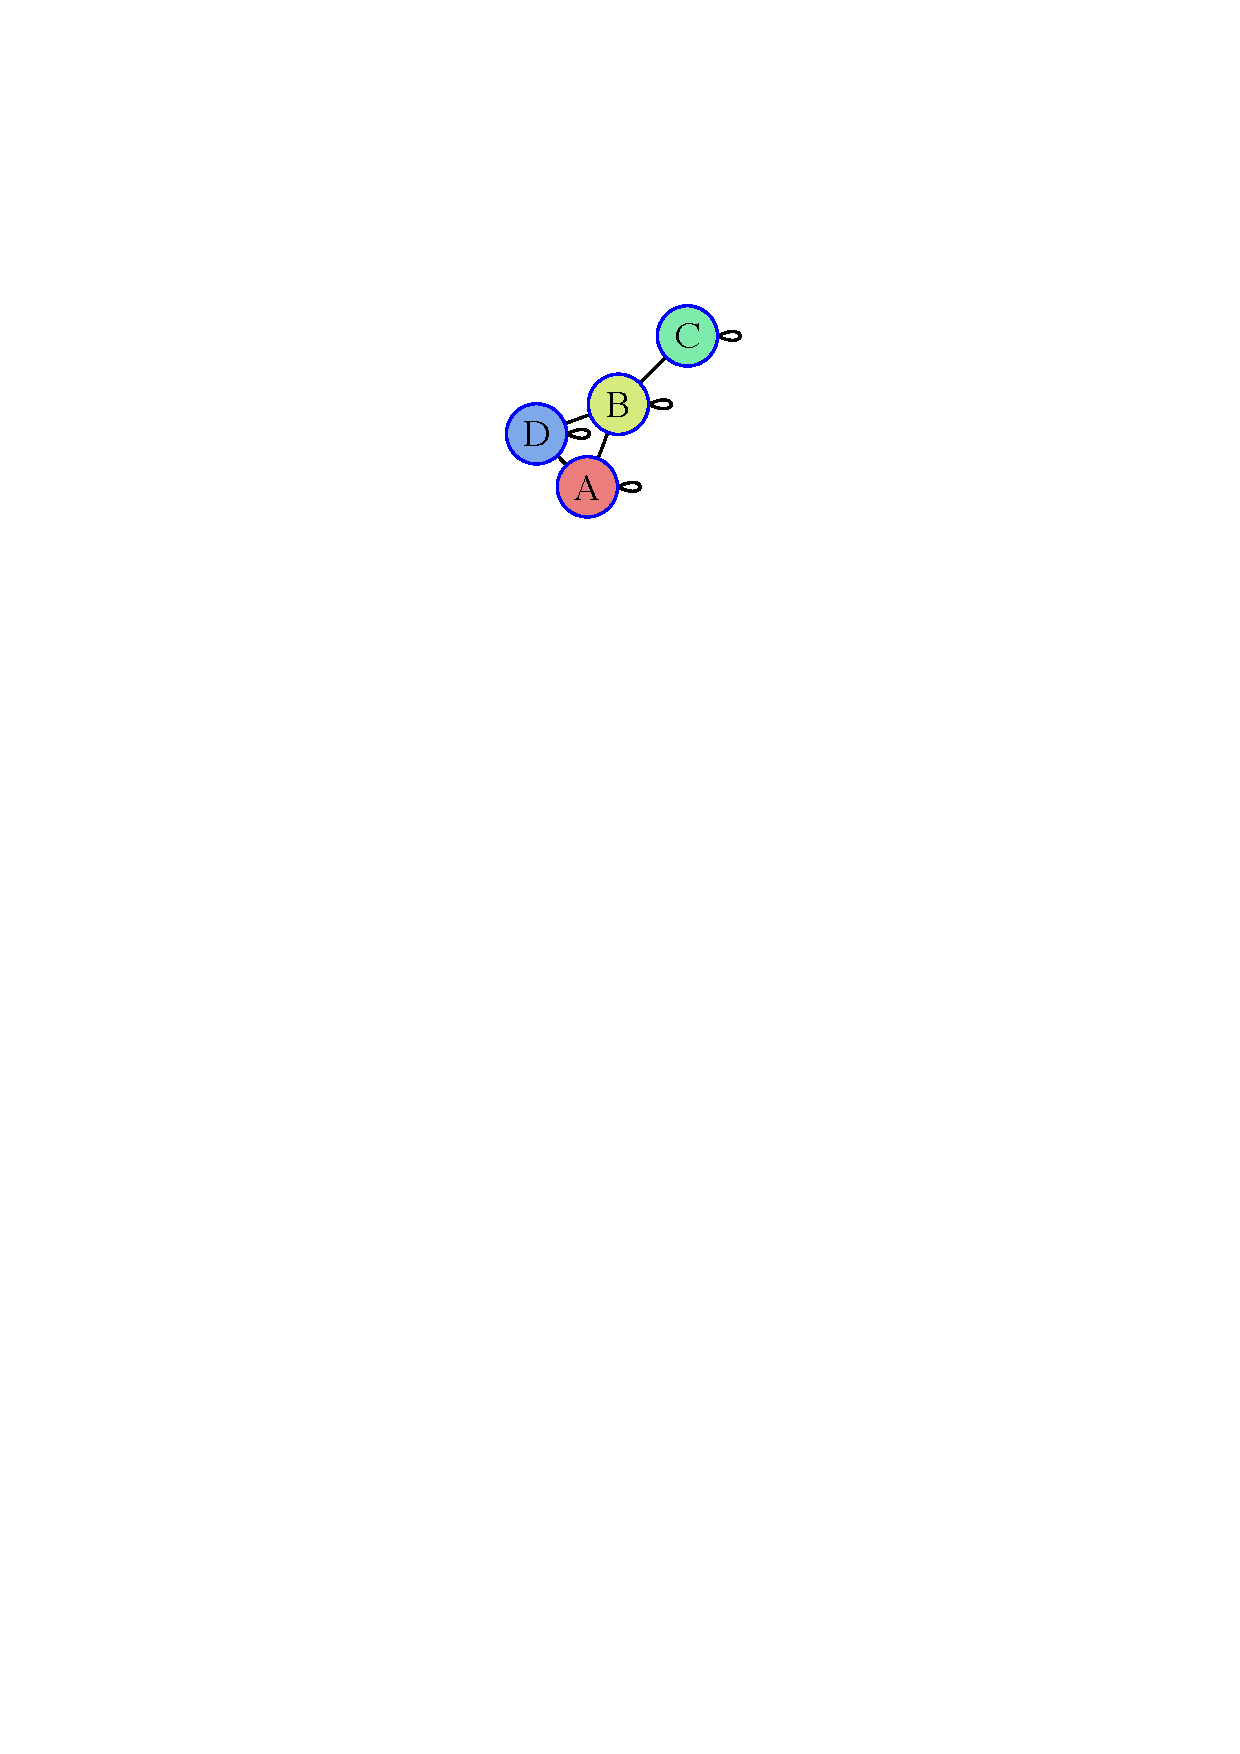
\includegraphics{img1.pdf}
\caption{\small{Ejemplo de comunidades con vínculos entre sí representados por nodos, donde A, B, C y D son comunidades. \cite{Clauset} denomina a esta agrupación como ``multigrafo''.}} \label{Grup1}
\end{figure}

\vspace{0.5cm}

Así pues, la matriz de adyacencia de este multigrafo tiene elementos $A'ij = 2me_{ij}$\footnote{Donde $e_{ij}=\frac{1}{2m}$ si $i$ y $j$ están conectados, y $e_{ij}=0$ si no lo están.}, donde la unión de dos comunidades $i$ y $j$ equivale a reemplazar las filas y columnas $i's$ y $j's$ por sus sumas, es decir, se trata de construir un vector que represente los vínculos del multigrafo (ver figura \ref{Grup1}). Esto implica que se debe encontrar un valor $\Delta Q{ij}$ en el cual el par $i, j$ maximizan el valor de $Q$ respecto a las demás combinaciones posibles. De esta manera, $\Delta Q_{ij}$ equivale a:

\begin{equation}
\Delta Q_{ij}=\left\{ \begin{array}{lc}
                         \frac{1}{2m}-\frac{k_ik_j}{(2m)^2} & \mbox{si}\,\,\,\, i\,\,\,\, \mbox{y}\,\,\,\, j\,\,\,\, \mbox{están conectados}\\
                          & \\
                          0 & \mbox{si}\,\,\,\, i \,\,\,\,\mbox{y}\,\,\,\, j\,\,\,\, \mbox{no } \mbox{están conectados}
                         \end{array} \right.
\end{equation}

\vspace{0.5cm}

Además, $a_i = \frac{k_i}{2m}$ es un vector de $\Delta Q_{ij}$ (note que la primera parte de la ecuación 4 puede ser re escrita como $\frac{1}{2m}-a_ia_j$).

\vspace{0.5cm}

De esta manera, el algoritmo se desarrolla mediante tres pasos:
\begin{enumerate}
\item Calcular los valores iniciales de $\Delta Q_{ij}$ y $a_i$ y establecer el elemento más grande de cada fila de la matriz $\Delta Q$ y se almacenarán en $H$\footnote{H es un vector que contiene el elemento más grande de cada fila de la matriz $\Delta Q_{ij}$ junto con las etiquetas $i$, $j$ del correspondiente par de comunidades.}.
\item Elegir el $\Delta Q_{ij}$ más grande de $H$, unir dicho valor a las comunidades correspondientes, actualizar la matriz de $\Delta Q_{ij}$, el cúmulo $H$ y $a_i$ e incrementar $Q$ en $\Delta Q_{ij}$.
\item Repetir el paso $2$ hasta qué surja una única comunidad.

\end{enumerate}


\subsubsection{Algortimo de \cite{Girvan1, Girvan2}}

El algoritmo de \cite{Girvan1, Girvan2} es uno de los métodos más conocidos para detectar comunidades, dado que permite considerar redes ponderadas y dirigidas. De manera puntual, este algoritmo consiste en eliminar progresivamente algunos vínculos del grafo total, en función a una medida especial de intermediación\footnote{Dicha medida se conoce como ``Edge Betweenness Centrality'' y es definida según el número de trayectorías más cortas entre dos nodos, que pasan por un vínculo.} que se calcula para cada uno de los enlaces del grafo. De esta forma, \cite{Girvan1, Girvan2} desarrollan su algoritmo mediante cuatro pasos:

\begin{enumerate}
\item Calcular la medida de intermediación para todos los vínculos del grafo.
\item Eliminar el vínculo que obtuvo el mayor valor de intermediación (por el que pasan un mayor número de trayectorias más cortas).
\item Volver a calcular la medida de intermediación para el resto de vínculos del grafo, en especial los afectados por la eliminación del enlace del paso anterior.
\item Repetir desde el segundo paso, hasta que no quede ningún vínculo.
\end{enumerate}

\vspace{0.5cm}

Como resultado se obtiene una estructura jerarquizada, en la que es posible definir distintos niveles de análisis para las comunidades. Ésta puede ser representada mediante un dendograma (figura \ref{dendo}), en el que cada nivel corresponde a los componentes separados restantes tras la eliminación del vínculo con mayor medida de intermediación, hasta llegar a un nivel de desagregación por nodos. Es por esto, como mencionan \cite{Girvan1, Girvan2}, que se requiere de un criterio adicional para saber cuál es el ``mejor particionamiento'', o cuándo las comunidades encontradas por el algoritmo son las mejores.

\begin{figure}[h!]
\centering
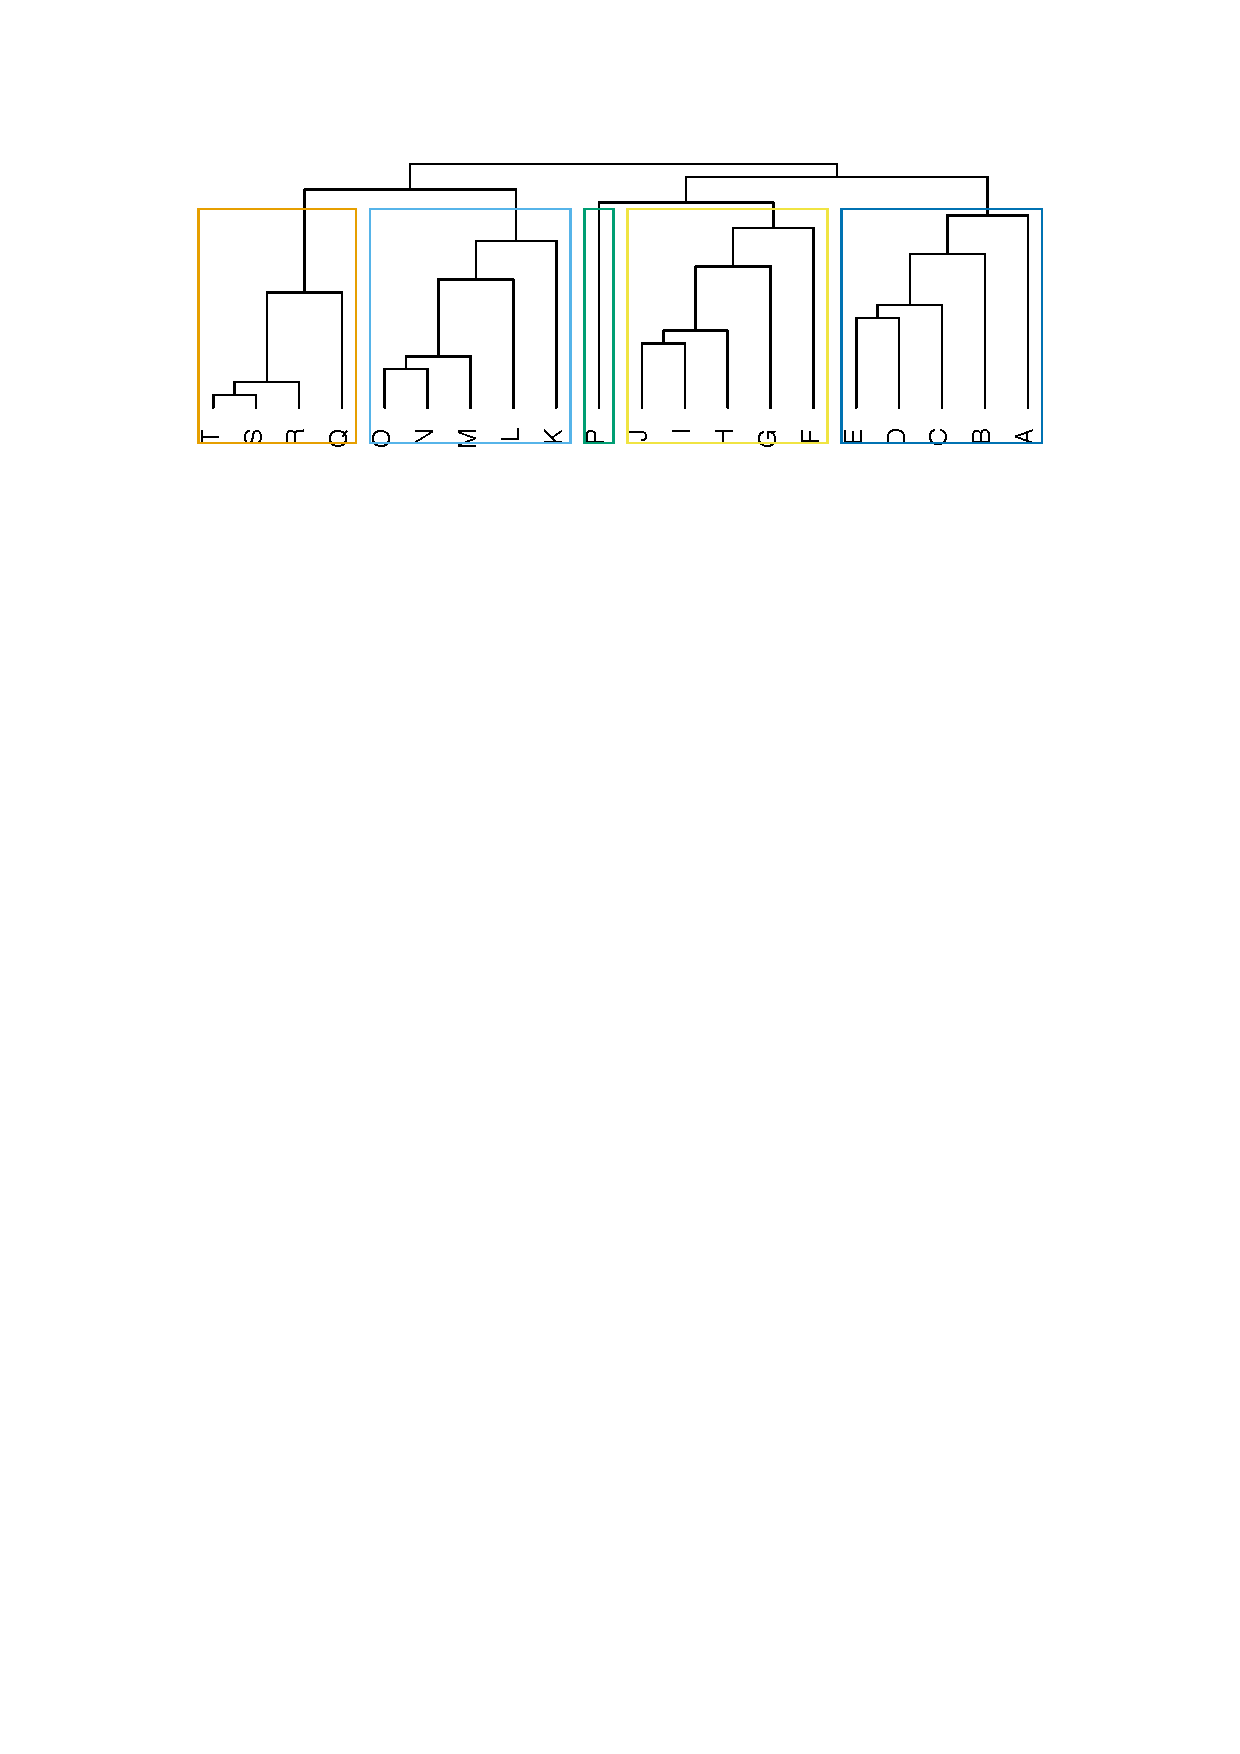
\includegraphics{Dendo.pdf}
\caption{\small{Dendograma de la red presentada en la figura \ref{Grup2} usando el algoritmo de \cite{Girvan1, Girvan2}.}} \label{dendo}
\end{figure}

El criterio adicional utilizado por \cite{Girvan1, Girvan2} para encontrar el número óptimo de comunidades consiste en maximizar una medida de modularidad. Dichos autores la definen como la fracción de vínculos en la red que conectan nodos de un mismo tipo --en el caso de redes ponderadas-- o simplemente un par de nodos --cuando la red no es ponderada-- , menos el valor esperado de la misma fracción si las conexiones fueran definidas de forma aleatoria. Esta medida (ecuación \ref{Ecu5}) puede tomar valores entre cero y uno, y entre mayor sea su valor se dice que la concentración de nodos sigue una estructura de comunidades. Análogamente, valores cercanos a cero indican que la ausencia de dichas agrupaciones debido a la predominancia de un proceso de vinculación aleatoria.

\begin{equation}
Q=\sum_i(e_{ii}-a^2_{i})=Tr(e)-||e^2||
\label{Ecu5}
\end{equation}

Donde, ``e'' corresponde a una matriz simétrica de tamaño $k\times k$, cuyos elementos $e_{ij}$ son fracciones de los vínculos que unen nodos de una comunidad $i$ con los de otra comunidad $j$; ``$a_i$'' corresponde a la fracción de vínculos que conectan nodos de una misma comunidad, y puede verse como una suma $a_i =  \sum_ie_{ij}$ de cada fila de la matriz $e$. Si la estructura de comunidades es fuerte, la traza de la matriz $eTr(e) =  \sum_i e_i$ tendrá valores cercanos a uno. Si la vinculación fuera aleatoria y no existieran agrupaciones en comunidades $e_{ij} = a_i \times a_j$, lo que permite reescribir la ecuación como la diferencia entre la traza de la matriz $e$, menos la suma de los elementos de la matriz $e^2$, denotada como $||e^2||$.

\vspace{0.5cm}

La medida de modularidad $Q$ es calculada tras la eliminación de cada vínculo con mayor valor de intermediación. En otras palabras, existe un valor de modularidad para cada uno de los niveles del dendograma. Así, se puede elegir la estructura ``óptima'' de comunidades, seleccionando el nivel que obtuvo un mayor valor de $Q$.

\subsubsection{Algoritmo de \cite{Pons}}

El algoritmo de \cite{Pons} puede ser considerado un algoritmo aglomerativo. Es decir, para la detección de comunidades no es necesario recurrir a eliminaciones de vínculos, ni a divisiones de subgrafos. El algoritmo de \cite{Pons} se conoce como ``Walktrap'', pues supone que al recorrer aleatoriamente un grafo, a través de sus vínculos, es posible quedar ``atrapado'' en sus componentes más densamente conectados, que se consideran comunidades. Para esto, definen dos medidas de distancia, que permiten capturar las similitudes estructurales entre nodos y comunidades. El algoritmo de \cite{Pons} se compone principalmente de seis procedimientos, que según los autores puede verse como un problema de agrupamiento (clustering), realizado en 6 pasos:

\begin{enumerate}
\item Elegir aleatoriamente un nodo v, que será el punto de partida del algoritmo y que representa una partición $P_1$, del total de nodos $V$, que conforman el grafo $G=(V,E)$.Es decir, $P_1 =\{\{v\},v \in V\}.$
\item Calcular todas las distancias entre todos los vértices adyacentes. Es decir, estimar cada una de las distancias $r_{vj}$, entre el nodo v y sus j vecinos (de orden 1).
\begin{enumerate}
\item A continuación se ejecuta el siguiente bucle, para cada una de las particiones $P$ que se definen en cada paso $k$. Es decir, $P_k = P_1, ..., P_n$.
\end{enumerate}
\item Elegir dos comunidades $C_1$ y $C_2$ en la partición $P_k$ de acuerdo con un criterio de distancia entre comunidades $r_{c1c2}$.
\item Unir las comunidades halladas en al paso anterior en $C_3 = C_1 \cup C_2$ y crear una nueva partición $P_{k+1} =(P_k\{C_1,C_2\})\cup\{C3\}$
\item Calcular y actualizar las distancias entre comunidades $r_{c1c2}$.
\item Repetir los procedimientos 3, 4, $n - 1$ veces hasta que se obtenga una partición que contenga todos los nodos del grafo. Es decir, hasta que $P_n = \{V \}$.
\end{enumerate}

El algoritmo de \cite{Pons} es más rápido que el de \cite{Girvan1, Girvan2} y es muy utilizado en redes de gran tamaño, a pesar de algunas de sus desventajas. En especial, no permite considerar grafos dirigidos, porque de otra forma sería difícil que el caminante aleatorio quedara ``atrapado'' en un componente denso. Además, el tamaño o número de pasos en cada trayectoria debe ser elegido de forma exógena, aunque se recomienda utilizar un valor entre $3$ y $5$, pues a mayor distancia disminuye la probabilidad de recorrer dos nodos que pertenezcan a una misma comunidad. Sin embargo, dicho algoritmo permite encontrar comunidades a diferentes escalas\footnote{Este problema es tratado por \cite{Leskovec1}, quienes encontraron que en grafos de más de cien nodos existe una relación inversa entre el tamaño de la comunidad y su ``calidad''. Es decir, las comunidades parecieran mezclarse o superponerse y la sola maximización de la modularidad no es suficiente para detectar pequeñas agrupaciones bien definidas, cuando se analizan grafos de gran tamaño.} e incluso los autores afirman que podría ser relevante para detectar comunidades superpuestas, algo que no es posible sólo maximizando la modularidad.

\subsubsection{Algoritmo de  \cite{Raghavan}}

También se conoce como ``label propagation community'' y la principal idea de este algoritmo subyace en los vecinos más cercanos --o nodos adyacentes-- que poseen los nodos, es decir, un nodo $x$ tiene $k$ vecinos $(x_1, x_2, ..., x_k)$ que portan una ``etiqueta'' que denota la comunidad a la que pertenecen. Entonces $x$ determina su comunidad de acuerdo a las ``etiquetas'' de sus vecinos. Así pues, se supone que cada nodo en la red opta por unirse a la comunidad a la que pertenecen el número máximo de sus vecinos, con vínculos rotos uniformemente al azar.

\vspace{0.5cm}

El proceso empieza con todos los nodos con etiquetas únicas donde las etiquetas se propagan a través de la red. A medida que las etiquetas se propagan, llegan a grupos de nodos densamente conectados que facilitan que aparezca rápidamente un consenso sobre una etiqueta única. Cuando muchos de estos grupos densos --o consensos-- se crean en toda la red, continúan expandiéndose hacia el exterior hasta los límites que sea posible hacerlo. Al final del proceso de propagación, los nodos que tienen las mismas etiquetas se agrupan juntos como una comunidad.

\vspace{0.5cm}

Este proceso se lleva a cabo de manera iterativa, en el cual en cada paso, cada nodo ``actualiza'' su ``etiqueta'' en base a las etiquetas de sus vecinos. De esta manera, el algoritmo se desarrolla en $5$ pasos:

\begin{enumerate}
\item Establecer las etiquetas en todos los nodos de la red. Para un nodo dado $x$, $C_{x}(0) = x$. Donde $C(u)$ es la etiqueta asignada.
\item Establecer $t = 1$.
\item Organizar los nodos de la red en un orden aleatorio y lo establecerlos en $X$.
\item Para cada $x \in X$ en un orden específico, sea $C_{x}(t) = f (C_{x_{i1}}(t),...,C_{x_{im}}(t),C_{x_{i(m+1)}}(t-1)$, $C_{x_{ik}} (t-1))$. $f$ aquí devuelve la etiqueta que se presenta con mayor frecuencia entre los vecinos y algunos vínculos se rompen de forma uniforme y aleatoria.
\item Si cada nodo tiene una etiqueta equivalente al número máximo de la que sus vecinos tienen, entonces se detiene el algoritmo. Si no, establecer $t = t + 1$ y correr desde el punto tres.
\end{enumerate}

%----------------------------------------------------------------------------------------------------------------------------------------------------------------------------------------------------------------------------------------------
%----------------------------------------------------------------------------------------------------------------------------------------------------------------------------------------------------------------------------------------------
%----------------------------------------------------------------------------------------------------------------------------------------------------------------------------------------------------------------------------------------------
%----------------------------------------------------------------------------------------------------------------------------------------------------------------------------------------------------------------------------------------------
\subsubsection{Algoritmo de Rosvall \citep{Rosvall1, Rosvall2, Rosvall3}} 
Éste algoritmo es desarrollado en \cite{Rosvall1}, \cite{Rosvall2} y \cite{Rosvall2} y es conocido como ``Infomap''. A diferencia de todos los algoritmos anteriores, éste algoritmo no busca maximizar una cualidad del corte o establecer un patrón de búsqueda intrínseca de los clusters, en lugar de ello, sus cimientos se encuentran en la teoría de la información de \cite{Shannon} donde el flujo de datos puede ser comprimido por un código que explota regularidades en el proceso que genera el flujo.


\vspace{0.5cm}

Como una proxy para el flujo de información los autores usan un caminante aleatorio, debido a que el caminante aleatorio utiliza toda la información en la representación de la red y nada más, es decir, es capaz de ``caminar'' por toda la red y captar toda la información sobre vínculos y nodos en toda la red (en términos de conexiones entre los nodos). Por lo tanto, proporciona un mecanismo predeterminado para generar una dinámica de un diagrama de red.

\vspace{0.5cm}

El problema de encontrar la mejor partición es expresada como la mínima cantidad de información necesaria para representar un caminante aleatorio en la red. Sí una partición tiene unos pocos vínculos inter-comunidad, es mas probable que el ``caminante'' permanezca dentro de la comunidad, dado que tendrá pocas ``salidas'' de la comunidad.

\vspace{0.5cm}

Así pues, el algoritmo busca una partición $M$, dentro de las $m$ particiones posibles, tal que minimize la longitud caminada por el caminante aleatorio. De manera formal, el algoritmo es expresado así:


\begin{equation}
L(M)=q H(Q) + \sum_{i=1} p_i H(P_i)
\label{Ecu5}
\end{equation}

\vspace{0.5cm}

Donde el primer término de la ecuación es la entropía inter-módulos y el segundo es la entropía intra-módulos. De forma puntual, $q$ es la probabilidad de que un caminante aleatorio ``salte'' de un módulo a otro\footnote{Entre menos conexiones tenga el módulo con le resto de la red dicha probabilidad será mas cercana a cero.}, $p_i$ es la fracción de movimientos intra-comunidad que ocurren en la comunidad $i$ más pa probabilidad de ``salir'' de la comunidad. $H(Q)$ es la entropía de los cluster y $H(P_i)$ es la entropía de los movimientos dentro del cluster.

%La estructura de la comunidad está representada entonces, a través de una nomenclatura de dos niveles basada en un proceso Huffman de codificación, es decir, un código para distinguir las comunidades en la red y otro para distinguir los nodos en las comunidades. 


\vspace{0.5cm}

%Cada nodo que es parte del mismo grupo M del nodo anterior se describe solamente con su sufijo, de lo contrario con prefijo y sufijo. A continuación, los sufijos se reutilizan en todos los prefijos, al igual que los nombres de calles se reutilizan en diferentes ciudades. La división óptima en diferentes prexifes representa la partición óptima de la comunidad.

%De forma general, en el primer nivel, el caminante aleatorio es ``soltado a caminar'' por la red, en el segundo nivel, se encuentra el mejor camino ``caminado'' por el caminante aleatorio y los módulos --o clusters-- donde éste quedó atrapado.

%----------------------------------------------------------------------------------------------------------------------------------------------------------------------------------------------------------------------------------------------
%----------------------------------------------------------------------------------------------------------------------------------------------------------------------------------------------------------------------------------------------
%----------------------------------------------------------------------------------------------------------------------------------------------------------------------------------------------------------------------------------------------

\section{Conceptos}
Esta sección cumple una función simple: empapar al lector del núcleo teórico de éste documento. Es necesario que establezcamos un concepto sólido de ``comunidad'' desde dos frentes: conceptual y pragmático. Con el primer frente se establecerá una definición de comunidad, con el segundo frente se mostrará como se clasifican las comunidades intrínsecamente de acuerdo al método empleado para hallarlas, por último será planteada una definición general de ``topología''.

\subsection{El Concepto de Comunidad} \label{ComuCo}
Una comunidad es una porción de una red en la cual existen más conexiones entre sus nodos que con el resto de la red \citep{Labatut, Leskovec2}. Por lo tanto, el concepto general de comunidad gravita alrededor de dos conceptos: cohesión y separación, donde el primero corresponde a las conexiones existentes dentro de la comunidad y el segundo a sus conexiones con el resto de la red \citep{Leskovec2}.

\vspace{0.5cm}


Una definición más formal sería: {\it ``un conjunto de nodos con alta densidad en los vínculos internos, mientras que en los vínculos externos baja densidad''} \citep{Lancichinetti}. Sin embargo, aunque la definición es exacta y general, la detección de dichas porciones más conectadas o densas en la red varía de algoritmo a algoritmo. La figura \ref{Grup2} muestra un grafo inicial y tres cortes de comunidades (particionamientos) de acuerdo a los algoritmos usados para detectarlas. De forma puntual, el particionamiento 1 corresponde al realizado por el algoritmo de \citep{Pons}, el particionamiento 2 al realizado por \citep{Girvan1, Girvan2}, el particionamiento 3 al realizado por el algoritmo de \citep{Blondel}

\vspace{0.5cm}

\begin{figure}[h!]
\centering
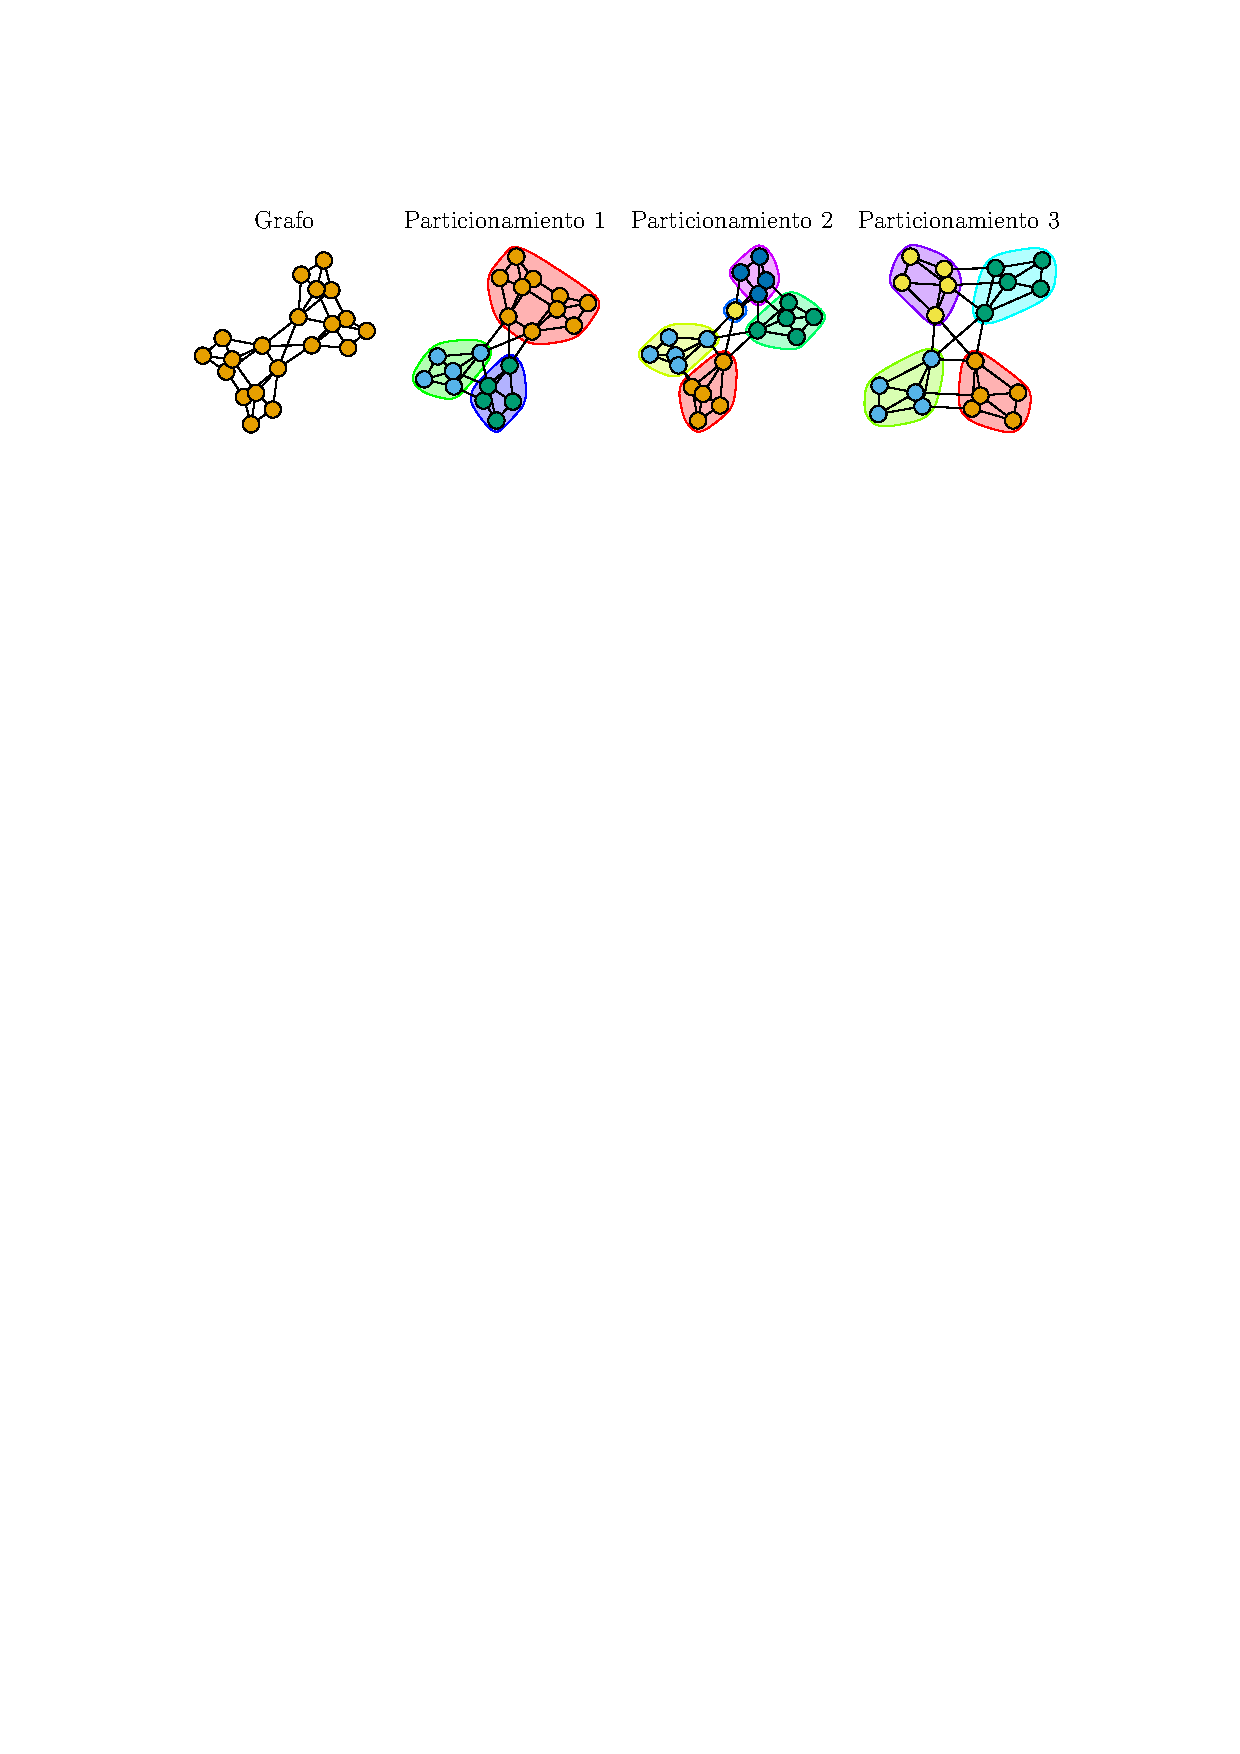
\includegraphics{ParticionesEj.pdf}
\caption{\small{Muestra de distintas comunidades a partir de una misma red.}} \label{Grup2}
\end{figure}

\vspace{0.5cm}

Es posible notar que cada particionamiento abarca distintos grupos de nodos y que cada comunidad es de distinto tamaño. Así pues, una comunidad puede definirse de acuerdo al algoritmo aplicado conservando la noción general ya presentada. Por ello, \cite{Labatut} y \cite{Orman} muestran algunas categorias de comunidades de acuerdo a los parámetros de los algoritmos:

\begin{enumerate}
\item \textbf{Densidad:} Es cuando una comunidad es definida propiamente a partir de valores de intra e inter conectividad de los cortes para medir la cohesión y separación respectivamente.
\item \textbf{Patrón:} Define la cohesión y la separación identificando subconjuntos (máximos) compuestos de pequeños patrones de interconexión específicos como ``cliques''. De esta manera, podría considerarse una comunidad como el patrón más grande identificado o un conjunto de patrones con nodos en común.
\item \textbf{Similaridad en los nodos:} Las nociones topológicas de cohesión y separación se establecen en términos de similitud entre los nodos de la comunidad (similitud intra-comunidad)\footnote{Teniendo en cuenta el conjunto de nodos adyacentes.} y no similitud entre los nodos de la comunidad con el resto de la red (no similitud inter-comunidad). En otras palabras, una comunidad se ve como un grupo de nodos que son similares entre sí, pero diferentes del resto de la red.
\item \textbf{Centralidad de los vínculos:} Los enlaces inter-comunidades tienen mayor índice de centralidad, ya que permiten conectar los nodos de una comunidad a los de otra, en comparación con los enlaces intra-comunidades. En otras palabras, la alta centralidad de enlaces inter-comunidad se refiere a la separación, y la baja centralidad de enlaces intra-comunitarios se refiere a la cohesión.
\item \textbf{Compresión:} Esta categoría no emplea los conceptos de cohesión y separación como todas las definiciones anteriores. En su lugar, adoptan una perspectiva de compresión de datos y tiene en cuenta la estructura de la comunidad como un conjunto de regularidades en la topología de la red que puede ser usado para representar toda la red de una manera más compacta. Por lo tanto, la mejor estructura de la comunidad es la maximización de la ``compacidad'' y la minimización de la pérdida de información.
\end{enumerate}


\subsection{Definición de los Algoritmos} \label{DefAlg}
Finalmente, una vez establecido el concepto de comunidad y habiendo presentado los algoritmos a evaluar, vamos a presentar en cuál de las cinco categorías presentadas en la sección \ref{ComuCo} se encuentra cada uno de los algoritmos a evaluar.

\vspace{0.5cm}

\begin{table}[h!]
\centering
\begin{tabular}{ll}
\textbf{Algoritmo} & \textbf{Tipo de Comunidad}\\ \hline 
   \cite{Blondel} & Densidad\\
   \cite{Clauset} & Densidad\\
   \cite{Girvan1, Girvan2}  &  Centralidad de Vínculos\\
    \cite{Pons}  &  Similarida en los nodos\\
    \cite{Raghavan}  & Densidad\\
    \cite{Rosvall1} & Compresión \\ \hline
\end{tabular}
\caption{\small{Categorías de los algoritmos a evaluar. Obtenidas de \cite{Labatut} y \cite{Orman}}}.
\end{table}

\vspace{0.5cm}

\subsection{El Concepto de Topología}
La topología de red es la estructura o la forma en que los nodos y vínculos se distribuyen y ordenan. Por ejemplo, en la figura \ref{TopoEj} es evidente la diferencia entre los grafos A, B, C y D. El grafo A es un grafo en ``estrella'', en el cual, un solo nodo central es quien tiene vínculos con los demás, el grafo B se conoce como grafo en ``anillo'', por su forma circular y en ciclo, podemos decir que no importa el nodo de éste grafo del que partamos, siempre volveremos a él al recorrer la red. el grafo C es una red en forma de árbol, en la que a partir de un nodo inicial (en este caso el nodo 1) comienzan a ser añadidos los demás nodos en orden jerárquico. Por último, el grafo D es una red completamente conexa, donde todos los nodos tiene vínculos unos con otros.

\begin{figure}[h!]
\centering
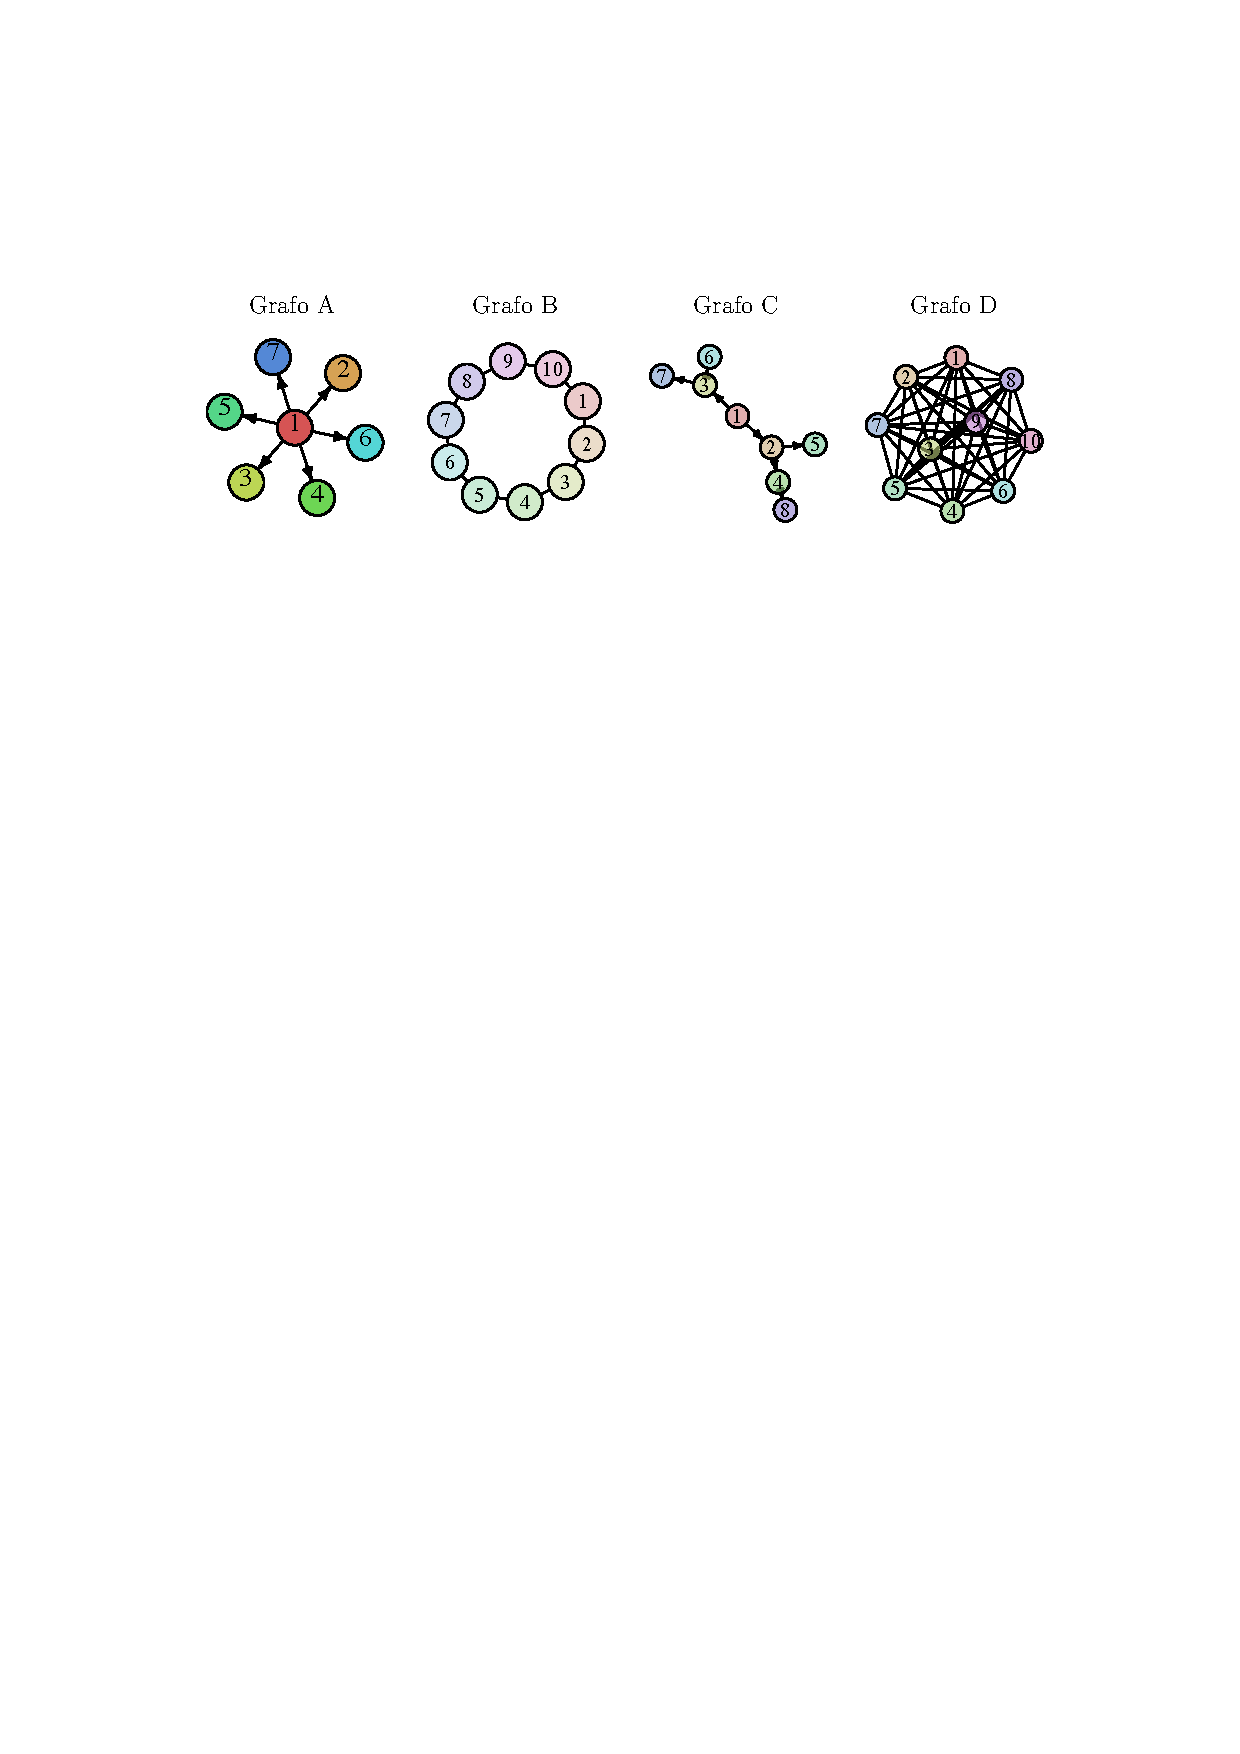
\includegraphics{TopoEj.pdf}
\caption{\small{Ejemplo de distintas topologías en redes.}} \label{TopoEj}
\end{figure}

\vspace{0.5cm}
El estudio de la topología de la red es de gran valor dado que permite ampliar el panorama estructural de la red para entender el mecanismo funcional de evolución de la red. No obstante, como ya se mencionó, en este documento sólo se harán cálculos de las estadísticas de la red, de modo que nos sea posible entender cuál es su topología y como es su comportamiento.

%------------------------------------------------------------------------------------------------------
\section{Hipótesis de Trabajo} \label{Hip}
%------------------------------------------------------------------------------------------------------

De acuerdo a lo presentado en la sección \ref{RedCitas} no se le ha prestado suficiente atención a las redes de citación en términos de diseñar --o encontrar-- un algoritmo capaz de reproducir cómo son las agrupaciones en las mismas. Durante el proceso de investigación ha surgido una pregunta crucial para la comprensión del mundo económico: ?`qué proceso lleva a que las redes de citas adopten la topología que tienen?\footnote{Sobre la topología de las redes de citas ver la sección \ref{TopoRed}.}.

\vspace{0.5cm}


Para llegar a responder --o encontrar-- lo que nos atañe en la investigación, es necesario comenzar a construir una base de fundamentos topológicos de la red. Durante dicho proceso surgió otra pregunta: ?`qué tipo de comunidad --en el contexto de la sección \ref{ComuCo}-- se forma en una red de citas?. Pues entender cómo se agrupan --o cuál es la mejor forma de entender el agrupamiento-- nos dará luz sobre el proceso subyacente de formación de redes de citas.

\vspace{0.5cm}

De acuerdo a la literatura en redes de citas, estás se forman por dos vías: vinculación preferencial y ``quién pega primero''\footnote{Una breve descripción de estos procesos se presenta en la sección \ref{ApGe}, por lo cual no se ve necesario ser exhaustivos en esta sección para mostrar la hipótesis principal de éste trabajo.}. Las comunidades que surgen bajo estos dos procesos presentarán comunidades del tipo ``centralidad de vínculos'', pues los agrupamientos se presentarán alrededor de unos cuántos nodos (artículos), lo que evidentemente aumentará el grado de intermediación de estos nodos. Pues los mayores componentes estarán vinculados por estos nodos.
\vspace{0.5cm}

Así pues, se busca contrastar si realmente en las comunidades encontradas por los diferentes algoritmos presentados prevalece como mejor algoritmo el del tipo ``centralidad de los vínculos''. Es decir,  si al comparar --usando los criterios de evaluación (ver sección \ref{Criterio})-- todo el conjunto de algoritmos que vamos a estudiar, resulta con las mejores medidas evaluativas el algoritmo del tipo ``centralidad de los vínculos''. Lo que sería igual a determinar si éste tipo de algoritmo es el mejor --del conjunto evaluado-- para detectar comunidades en redes de citas\footnote{Note que la hipótesis presentada está enlazada al párrafo anterior a éste.}.


\section{Metodología}


En esta sección primeramente se muestra el criterio bajo el cual se van a evaluar los algoritmos planteados en la sección \ref{EvAl}, a continuación, se exponen los conceptos teóricos y matemáticos de los criterios de comparación. Luego, se mostrará cómo se construyó la base de datos empleada y cómo está compuesta. Finalmente, se realizará una breve introducción al tipo de red que se usa en este estudio.

\subsection{Criterio de Comparación de Algoritmos} \label{Criterio}

Siguiendo lo planteado por \cite{Gleich}, \cite{Leskovec1, Leskovec2} y \cite{Yang}, existen dos maneras de evaluar la eficacia de los algoritmos al momento de detectar comunidades. La primera forma es contrastando las comunidades encontradas en la red con las comunidades reales y observar si ambas coinciden o no. La segunda forma es tratar de obtener algún tipo de ``verdad fundamentada''\footnote{Del inglés ``Ground-Truth''.}, en cuyo caso el conjunto de nodos --o comunidad-- arrojado por el algoritmo pueden ser calificados (respecto a la calidad de la comunidad) por dicha medida. Esta ``verdad fundamentada'' o medida para evaluar algoritmos es denominada ``conductancia''\footnote{Del inglés \emph{``conductance''}. La palabra no tiene traducción del inglés, por ello se propone ``conductancia'' como la mejor traducción de la palabra.} (o métrica normalizada del corte) que es una medida de la calidad de la comunidad, es decir, muestra que las mejores comunidades están densamente unidas en conjuntos de nodos conectados al resto de la red a través de unos pocos vínculos. No obstante, y como se podrá observar más abajo, las redes de citaciones siguen un patrón específico de formación por lo cual fue necesario modificar la métrica a la topología de la red planteada.

\vspace{0.5cm}

En esta investigación se usará la \emph{conductancia} y la modularidad como medidas para determinar cuál de todos lo algoritmos evaluados realiza mejores cortes en la red de citaciones. Especificamente, un pequeño valor de \emph{conductancia} y un valor grande de la modularidad indicarán una estructura de comunidad fuerte\footnote{Aunque la razón de los valores deseables para ambas medidas es explícita en la sección 5.1.1 y 5.1.2, el lector ya debe suponer que las medidas propuestas tienen valores que nos indican que tan buena es la calidad del corte realizado sobre la red, en el caso de la \emph{conductancia}, un corte perfecto equivaldría a que su valor sea igual --o sea lo más cercano-- a cero. Por otro lado, en el caso de la modularidad, el mejor corte se evidencia en cuanto su valor sea lo más cercano --o igual-- a uno.}. Para este fin, se usará el software estadístico R, de manera puntual, la librería en análsis de redes ``igraph'' \citep{Csardi}. La métrica \emph{conductancia} se construyó a partir de las funciones de control incluidas en el software estadístico R, dado que ni el software ni el paquete incluían estas medidas según lo propuesto por \cite{Leskovec1, Leskovec2} y \cite{Yang}; la métrica modularidad  ya se encontraba en las funciones incluidas en el paquete según lo propuesto por \cite{Girvan1, Girvan2}, \cite{Leskovec1, Leskovec2} y \cite{Yang}.

\vspace{0.5cm}

La razón por la cuál se usarán estas dos medidas, es porque ambas medidas sirven como complemento para la calidad del corte  \citep{Gleich}. %La \emph{conductancia} realiza métrica de aprendizaje \emph{no supervisado} y la modularidad podría clasificarse como una métrica \emph{supervisada}. Por lo tanto, al evaluar los algoritmos con estas dos medidas estamos evitando sesgar la evaluación al utilizar una medida \emph{no supervisada} y otra \emph{supervisada} \citep{Leskovec1, Leskovec2}. 
Aunque ambos criterios miden lo mismo, sus métodos de medición difieren en muchos aspectos. Por lado, la conductancia \emph{cuenta} los vínculos intra e inter comunidades sin imponer un punto de comparación, es decir, es una medida \emph{no supervisada}\footnote{En términos estadísticos, podemos clasificar los análisis en dos campos: \emph{supervised learning} y \emph{unsupervised learning}. El primer campo se caracteriza por realizar una exploración de los datos a partir de un modelo teórico en mente, el segundo por explorar los datos y permitir que estos hablen. En este orden, la \emph{conductancia} es un métrica no supervisada, pues solo cuenta los vínculos intra e inter comunidad, y la modularidad --dado que impone un punto de comparación para el corte realizado-- sería una métrica supervisada.} pues solo explora los cortes en términos de vínculos, por otro lado, la modularidad genera una red aleatoria --conservando el grado de los nodos de la red inicial-- y compara las comunidades de ambas redes (la red aleatoria y la red inicial), es decir, supone que el mejor particionamiento posible es el de la red aleatoria y lo compara con el realizado en la red inicial, si ambas redes son idénticas la medida será igual a 1. Así pues, ambos criterios son medidas complementarias dado que usando las dos medidas se abarca tanto el análisis no supervisado como el análisis supervisado de la calidad del corte \citep{Yang}. 

\vspace{0.5cm}

A modo complementario de esta breve introducción a las medidas usadas, se presentará una breve revisión de literatura de las medidas y sus respectivas formalizaciones para la aplicación a redes.

\subsubsection{Modularidad}

No existe una formalización matemática única para determinar la modularidad \citep{Newman4} y el lector ya se habrá dado cuenta de ello al haber leído la sección \ref{EvAl}. No obstante, es importante que se establezca el concepto que está detrás de las diferentes formalizaciones.

De forma general, podemos definir la modularidad como una medida de la calidad del corte o la fuerza de la estructura encontrada por el algoritmo al dividir la red en comunidades \citep[Cap. 7]{Newman6}. Dicha ``calidad'' del corte es medida al comparar la probabilidad de tener vínculos que están dentro de las comunidades en la red menos la probabilidad esperada en una red equivalente (caso nulo) con el mismo número de nodos, con los vínculos asignados de forma aleatoria, manteniendo el grado de los nodos. Si la medida es positiva\footnote{El valor de esta medida se encuentra en el intervalo $[\frac{-1}{2},1)$.}, entonces el número de nodos dentro de los cortes supera el de los nodos distribuidos de forma aleatoria.

\vspace{0.5cm}

De manera puntual, la medida de modularidad que se usará en este documento es la misma usada por \cite{Yang}, \cite{Girvan2} y \cite{Newman4}:

\begin{equation}
 f(S)=\frac{1}{4}(m_{S}-E(m_s))
 \end{equation}
 
Donde $S$ es un conjunto de nodos, $m_S$ es el número total de vínculos entre los nodos de $S$ y $E(m_S)$ el número esperado de tales vínculos en un grafo conservando el grado de los nodos de la red inicial.

\vspace{0.5cm}
Se usará la medida de \cite{Yang}, \cite{Girvan2} y \cite{Newman4} porque es la más simple y es además la usada por \cite{Leskovec1} como complemento para sus evaluaciones.

\subsubsection{\emph{Conductancia}}

De acuerdo a la definición dada por \cite{Leskovec2}, la \emph{conductacia} es {\it ``la noción más simple de la calidad del agrupamiento, ya que puede simplemente ser considerada como la relación entre el número de vínculos dentro de la agrupación y el número de vínculos que están fuera del cluster''}. Dicha medida es usada para capturar cuantitativamente una comunidad de acuerdo a una noción de orden, es decir, las mejores comunidades son aquellas que están mejor conectadas internamente en lugar de externamente. Esto es, entre menos vínculos tenga una comunidad --o más apartada se encuentre-- con el resto de la red, será de mejor calidad.

\vspace{0.5cm}

De acuerdo a lo planteado por \cite{Yang}, la \emph{conductancia} --que mide la fracción del volumen total de vínculos que se encuentran fuera del cluster-- la definimos así:

\begin{equation}
f(S)=\frac{c_S}{2m_S + c_s}
\end{equation}

Donde $c_S$ es el número de vínculos que se encuentran en el límite --o periferia-- de $S$.

\subsection{Muestra de Datos}

Se utiliza una muestra de datos de citaciones construida desde la base de datos RePEc de dominio público obtenida por medio de ``web scrapping'' en formato JSON\footnote{JavaScript Object Notation.} y procesados en Python usando las librerías ``pandas'', ``beautifulsoup'' y ``numpy'', y depurada en el software estadístico R por medio de la librerías ``plyr'' y ``dplyr''. La base de datos se construyó partiendo de 32 artículos incluidos en el libro ``Rational Expectations and Econometric Pactice'' editado por \cite{Lucas2}.

\vspace{0.5cm}

?`Porqué los artículos en dicho libro los consideramos como el núcleo base para la construcción de las redes de citas? Porque el libro de Lucas y Sargent es la selección, hecha por dos de los revolucionarios más respetados, de los artículos más influyentes de la formación de la nueva economía clásica, es decir, son los artículos que los autores consideraban los más valioso dentro de la nueva economía clásica. {\it ``Aún más: eran su predicción acerca de cuáles habrían de ser los más importantes para el desarrollo de la revolución en marcha''} \citep[Pág. 48]{Salazar1}.

\vspace{0.5cm}

El proceso de depuración se desarrolló en dos etapas: primero se eliminaron todas las citas duplicadas teniendo como referencia el nombre del articulo, es decir, sí en la base de datos habían dos citas (filas) que contenían los mismos artículos en el mismo orden, es decir, que $x$ es citado por $y$ en ambos casos (los casos donde $x$ cita a $y$ y $y$ cita a $x$ eran ignorados) entonces una cita sería eliminada. En esta instancia, la base de datos perdió más de la mitad de sus datos (ver cuadro \ref{c2}). Después, se aplicó la segunda depuración, la cual consistía en buscar por nombre de autores y años de publicación duplicados o inconsistencias\footnote{Tales como un autor que publicó varios artículos en un mismo año pero que en el ID queda registrado como si todos esos artículos fuesen el mismo. Por ejemplo, Thomas Sargent publicó en 1976 3 artículos distintos, no obstante, el ID para los tres es ThSa1976, en este paso entonces se modificaba cada ID para que en las redes pudiera identificarse que eran 3 artículos distintos añadiendo al final del ID letras para identificar sus diferencias, por ejemplo: ThSa1976a, ThSa1976b y ThSa1976c.} y eliminarlas o corregirlas respectivamente. La base de datos de citas de \cite{Lucas1} ya había sido construida para la investigación en \citep{Salazar1} por lo tanto solo era necesario añadirla a la base actual.

\vspace{0.5cm}

\begin{table}[h!]
\centering
\begin{tabular}{lr}
\textbf{Proceso} & \textbf{Número de datos}\\ \hline 
   Datos iniciales & 346108\\
   Primera depuración & 97750\\
   Segunda depuración  &  82944\\
    \cite{Lucas1}  &  791\\
    Base total  & 83735 \\ \hline
\end{tabular}
\caption{\small{Resumen del proceso de depuración}.} 
\label{c2}
\end{table}

\vspace{0.5cm}

El cuadro \ref{c3} muestra la evolución en términos acumulativos de los nodos y vínculos que aparecen en cada año en la red estudiada, lo que permite concluir en términos de \cite{Barabasi1} que se trata de una red \emph{libre de escala} pues el número de vínculos a partir de 1980 es el doble --o más-- que el número de nodos añadidos en cada periodo. 

\vspace{0.5cm}

\definecolor{LightBlue}{rgb}{0.5,0.8,0.7}
\begin{table}[h!]
\centering
\resizebox{10cm}{!} {
\begin{tabular}{cccccc}
Año & Nodos & Vínculos & Año & Nodos & Vínculos\\ \hline 
1976 & 22   & 26   & 1995   &  3037  & 6067 \\
1977 & 41   &  47   & 1996  &   3686 & 7355 \\
1978 & 67   & 89    & 1997  &  4407  & 8786  \\
1979 & 102 & 147  & 1998  & 5292   & 10686 \\
1980 & 159 & 243  & 1999  & 6319   & 12927\\
1981 & 208 & 368  & 2000 & 7520    & 15649\\
1982 & 296 & 552 &  2001 & 8862    & 18837 \\
1983 & 367 & 724  & 2002 & 10479  & 22634\\
1984 & 471 & 920  & 2003 & 12249  & 26828\\
1985 &579  & 1100 & 2004 & 14430 & 31945\\
1986 & 721 & 1425 & 2005 & 16828 & 37579\\
1987 & 840 & 1681 & 2996 & 19348 & 43420\\
1988 & 990 & 2016 & 2007 & 21808 & 49198\\
1989 & 1192 & 2451 & 2008 & 24358 & 55046\\
1990 & 1376 & 2487 & 2009 & 26900 & 60548\\
1991 & 1635 & 3356 & 2010 & 29318 & 65610\\ 
1992 & 1886 & 3800 & 2011 & 32146 & 71306\\
1993 & 2186 & 4354 & 2012 & 35111 & 77248\\
1994 &  2497 & 4934 & 2013  & 38321 & 83735 \\ \hline
\end{tabular}}
\caption{\small{Evolución citas en términos acumulativos de nodos y vínculos. Construcción propia.}}
\label{c3}
\end{table}

\vspace{0.5cm}
En total se contará con 83748 citas correspondientes al periodo 1976-2013 (38 años) que no solo corresponden a citas de los 32 artículos contenidos en el libro de \citep{Lucas2}, de esta manera: para las citas de 1976 solo se contaba con los artículos del libro de \cite{Lucas2}, obteniendo citas de la siguiente forma $i\rightarrow j$ (donde $j$ son los citantes de 1976 e $i$ los artículos iniciales extraídos de \citep{Lucas2}), para 1977 se cuenta con los artículos i más los artículos $j$ (es decir, aquellos que citaron a los artículos $i$ en 1976) y los artículos $l$ que son los citantes de 1977, obteniendo citas de la forma $i\rightarrow l$ y $j\rightarrow l$. En 1978 se cuentan los artículos $i$, $j$ y $l$ más los citantes $p$ que corresponden a los artículos nuevos (es decir, los correspondientes a 1978), dando lugar a citas de la forma: $i\rightarrow p$, $j\rightarrow p$ y $l \rightarrow p$ y así sucesivamente para los años posteriores.

\vspace{0.5cm}

La muestra de datos construida en total está compuesta por 38321 nodos y 83735 vínculos, además, es propiedad del grupo de investigación COAPTAR y fue usada con autorización de los correspondientes propietarios.


\subsection{Red de Citas: Aproximación General} \label{ApGe}

Las redes de citación consisten en un conjunto de artículos (nodos) que son citados por otros artículos. La representación de una cita se computa cómo un vínculo dirigido de la forma $i \rightarrow j$ (ver figura \ref{cita}), es decir, el artículo $i$ es citado por el artículo $j$.

\vspace{0.5cm}

\begin{figure}[h!]
\centering
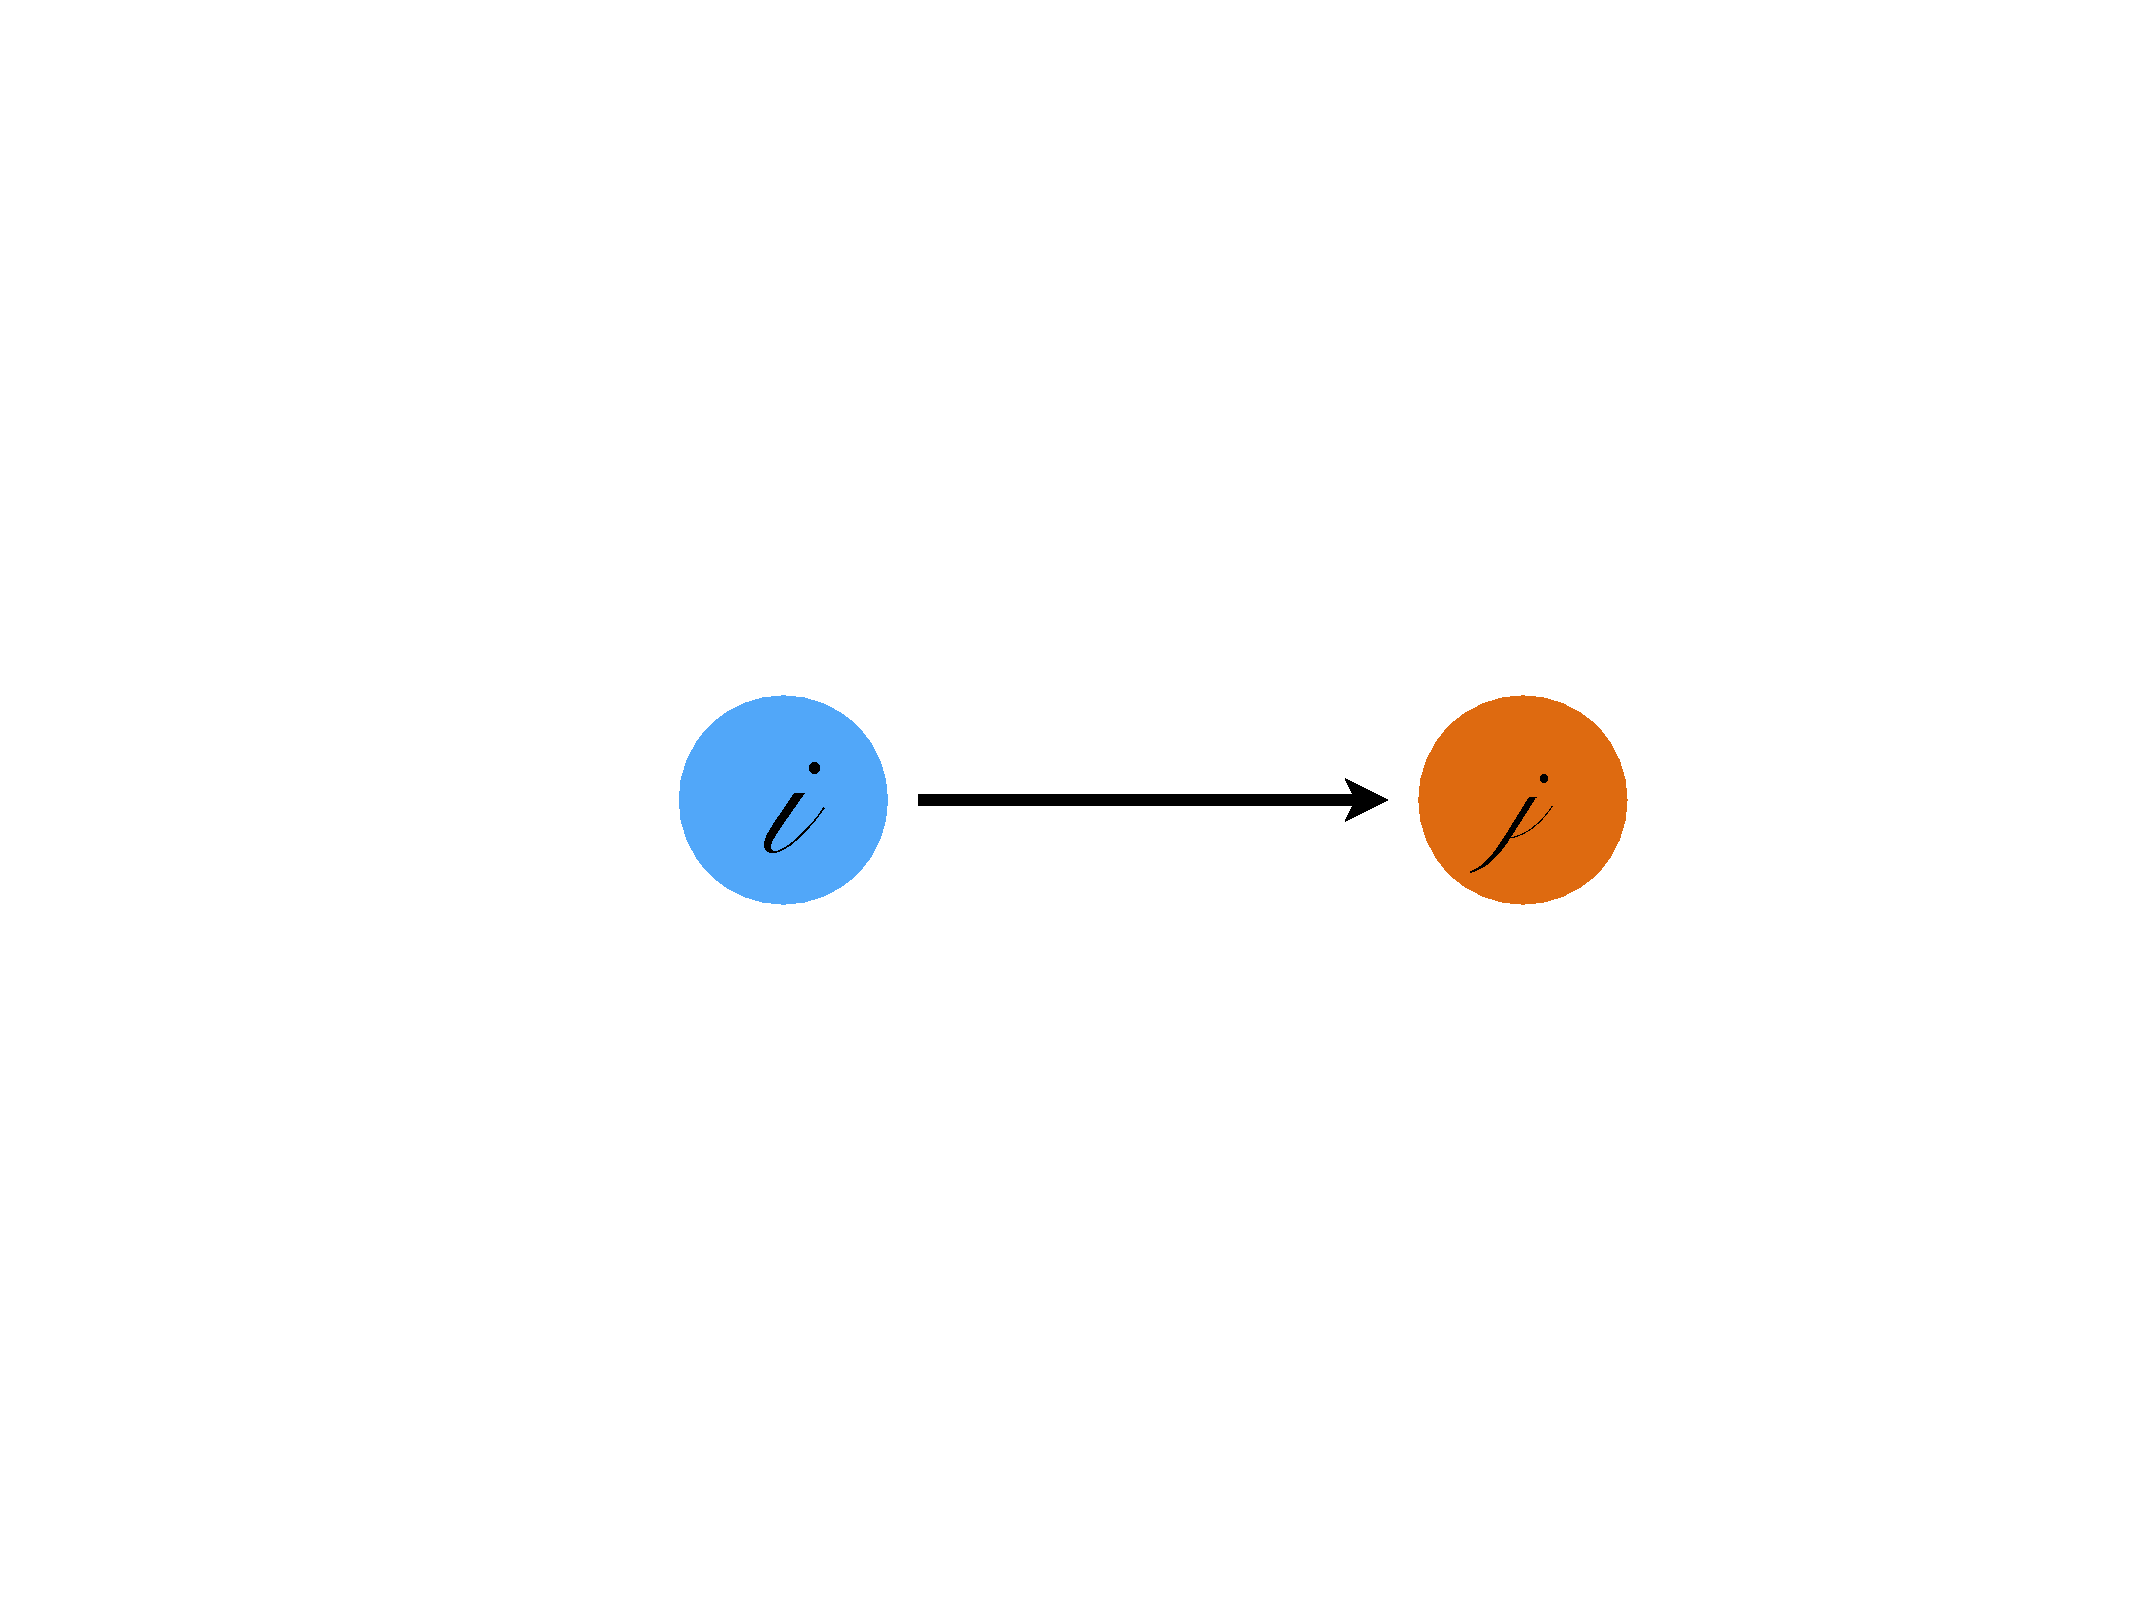
\includegraphics[scale=0.5]{Citaf.pdf}
\caption{\small{Representación en redes complejas de una cita.}} \label{cita}
\end{figure}

\vspace{0.5cm}

El vínculo dirigido establece dos características para el entendimiento e interpretación de la red  \citep{Salazar1}: \emph{i.)} en términos ontológicos, el contenido del segundo artículo ($j$) es influenciado por el contenido primer artículo ($i$); \emph{ii.)} en términos temporales, el vínculo dirigido establece que el segundo artículo ($j$) es precedido por el primer artículo ($i$).

\vspace{0.5cm}

De forma general, una red de citas sigue un patrón simple: redes dirigidas en estrella que se conectan unas a otras por uno o más vínculos (la figura \ref{DosRed}.A es un ejemplo de una red dirigida en estrella). Por supuesto, en este caso, con ``redes en estrella'' también nos referimos al tipo de vínculo más simple existente en un grafo: una diada\footnote{Una diada es el tipo de vínculo que tiene un nodo con otro, es decir, una conexión entre dos nodos (ver figura \ref{cita}).}.

La figura \ref{DosRed}.B muestra una posible red de citaciones en su expresión más simple. Cada área resaltada muestra un subgrafo en forma de estrella y cómo se conecta por medio de un único vínculo con otro subgrafo que posee la misma forma donde el nodo central de cada estrella se resalta de color distinto al del resto de la red.

\vspace{0.5cm}

\begin{figure}[h!]
\centering
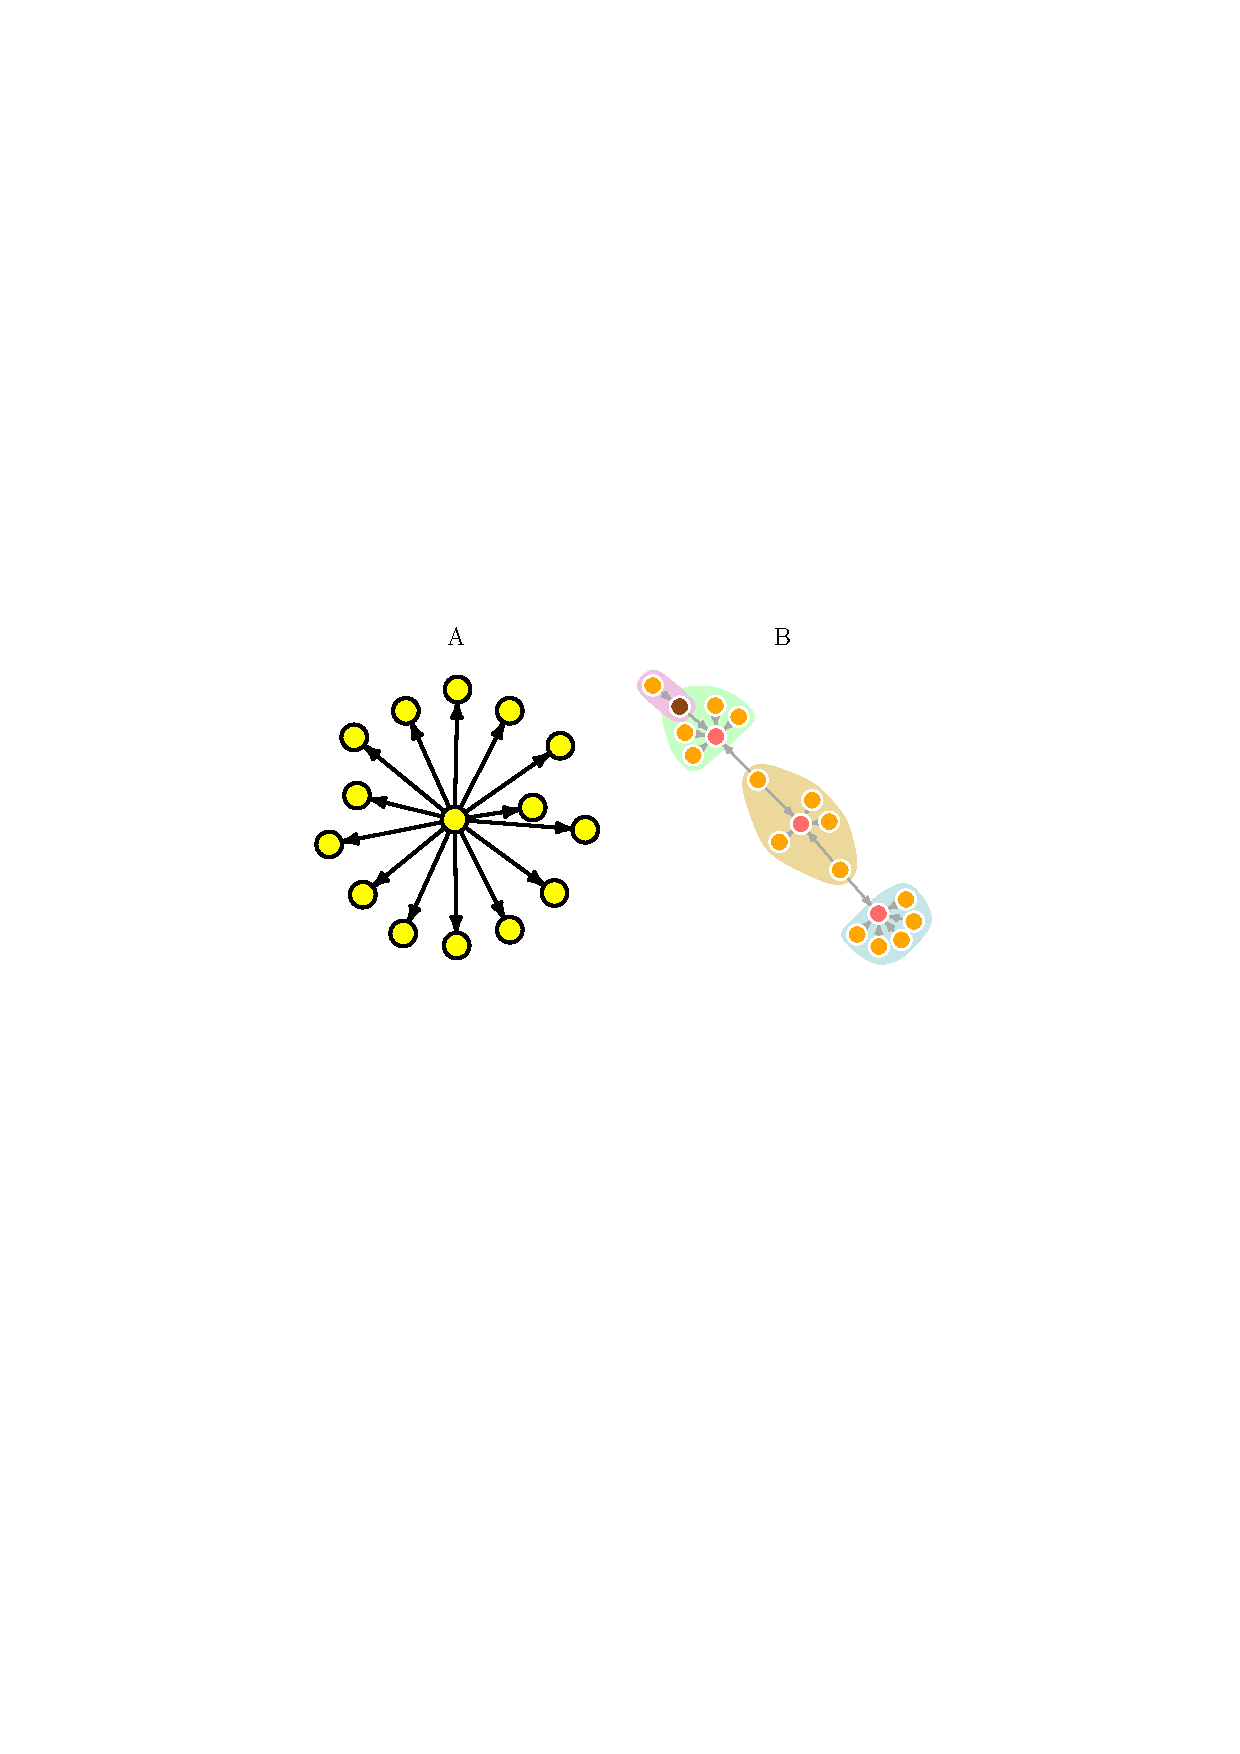
\includegraphics{DosRed.pdf}
\caption{\small{Red con topología en forma de estrella (derecha) y simulación de red de citas como el conjunto de redes en estrella unidas mediante un vínculo (izquierda).}} \label{DosRed}
\end{figure}

\vspace{0.5cm}

La figura \ref{DosRed}.B es una versión muy simplificada del aspecto de una red de citas en la realidad. En contraste, la figura \ref{1980} es una versión exacta de una red de citas de la realidad. Es posible observar a simple vista la formación de algunos ciclos o cierres triádicos, no obstante, la frase ``cierres triádicos'' no expresa de forma exhaustiva el tipo de ciclo que se presenta en la red, dado que es posible ver ciclos compuestos hasta por 4 nodos.

\vspace{0.5cm}

\begin{figure}[h!]
\centering
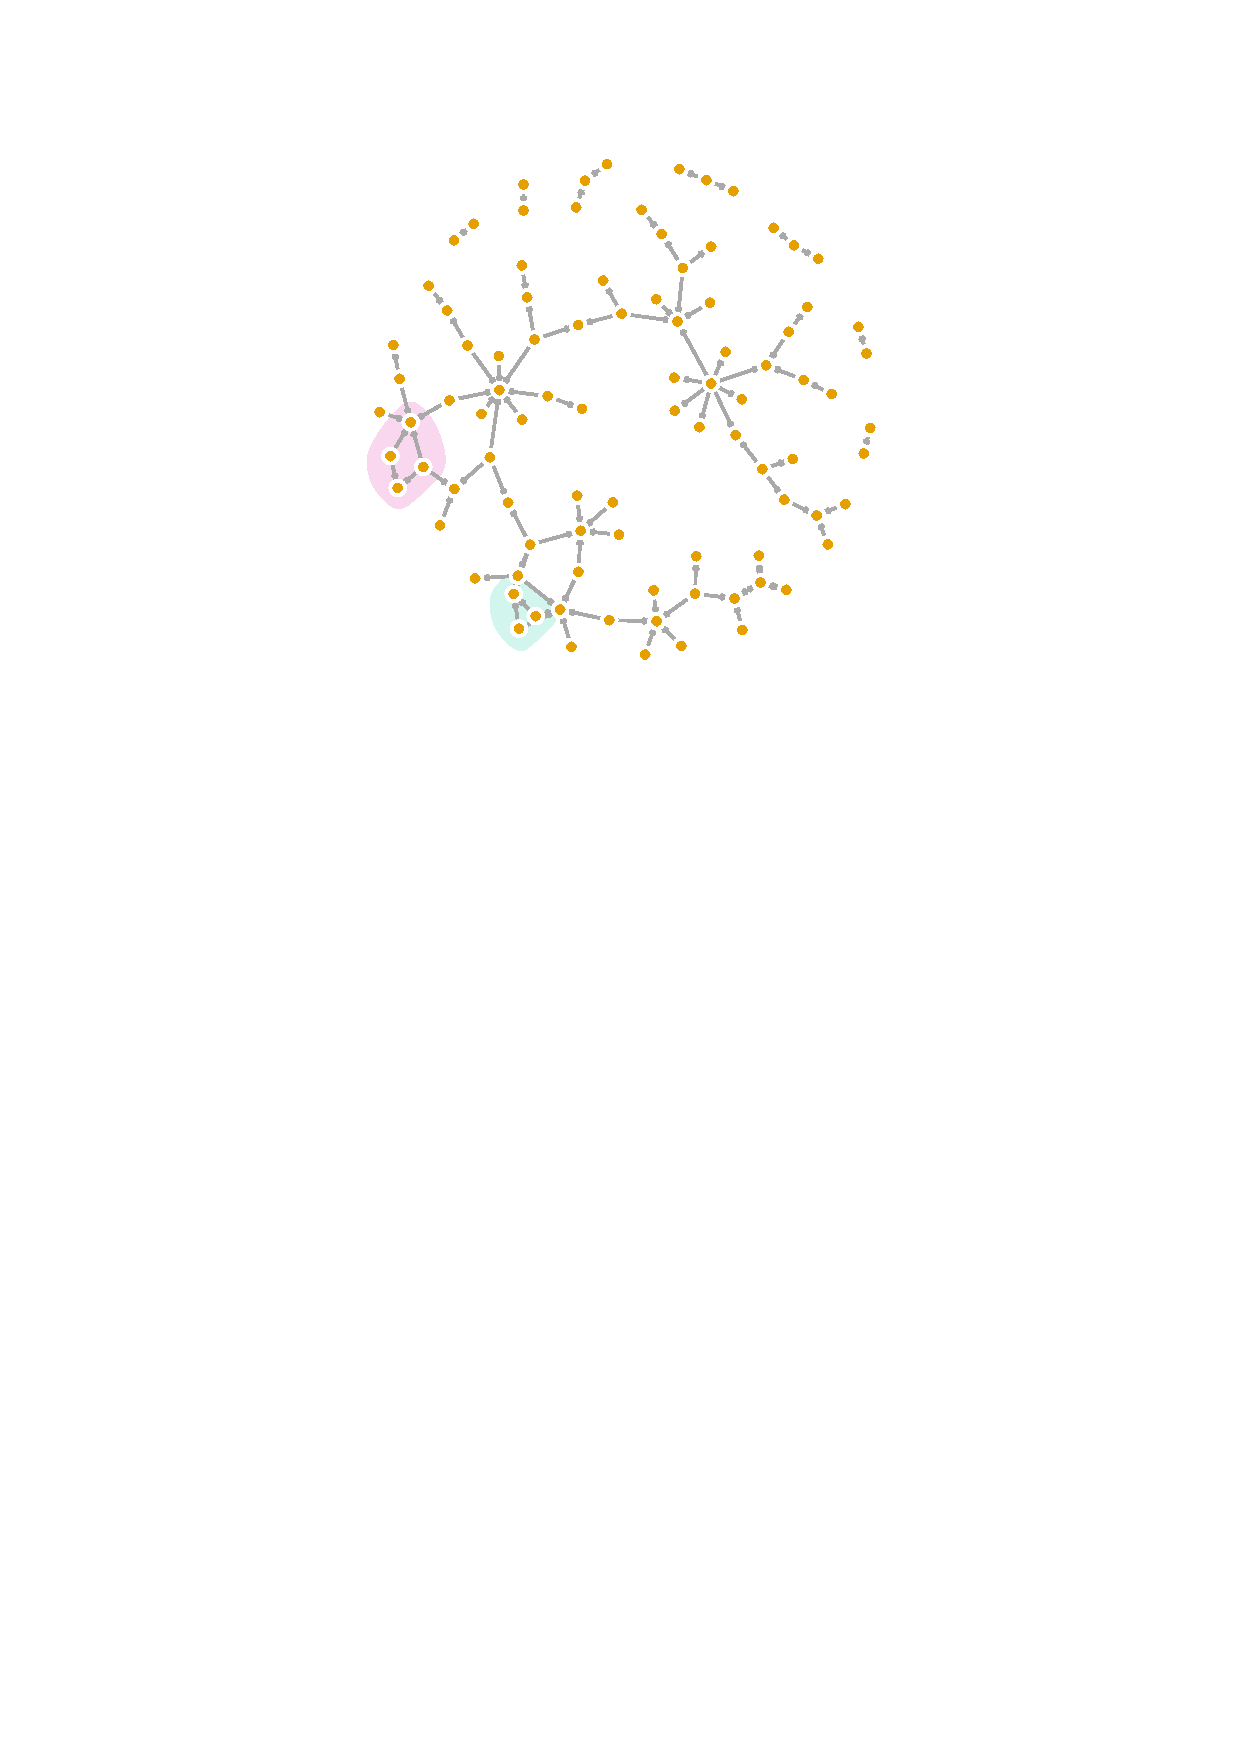
\includegraphics{1980.pdf}
\caption{\small{Porción de la red estudiada correspondiente a 1980.}} \label{1980}
\end{figure}

\vspace{0.5cm}


Estos ciclos dan a luz ``estrellas deformes'' dentro de la red pero que a la vez hacen más denso el componente implicado, además, nos ``habla'' sobre la dinámica de la formación topológica de la red. Hemos entendido que las redes de citas en general son redes dirigidas con forma de estrella, no obstante, hemos conocido que las estrellas pueden tener ciclos o ``deformidades''. Las estrellas deformes se forman debido a la restricción temporal de las citaciones, es decir, no es posible que un nodo (artículo) que aparece en $t_{0}$ forme un vínculo\footnote{Es decir, que cite a dicho artículo.} con un nodo que apareció en $t_{2}$, si es posible que un nodo que aparece en $t_{n+1}$ forme un vínculo con un nodo que apareció en $t_{0}$ y $t_{n}$. 

\vspace{0.5cm}

La figura \ref{estdef} muestra un ejemplo simple de las estrellas deformes. De manera puntual --y como ya se mencionó-- las deformidades en las estrellas se forman por los ciclos formados por la dinámica de la formación de las citaciones.

\begin{figure}[h!]
\centering
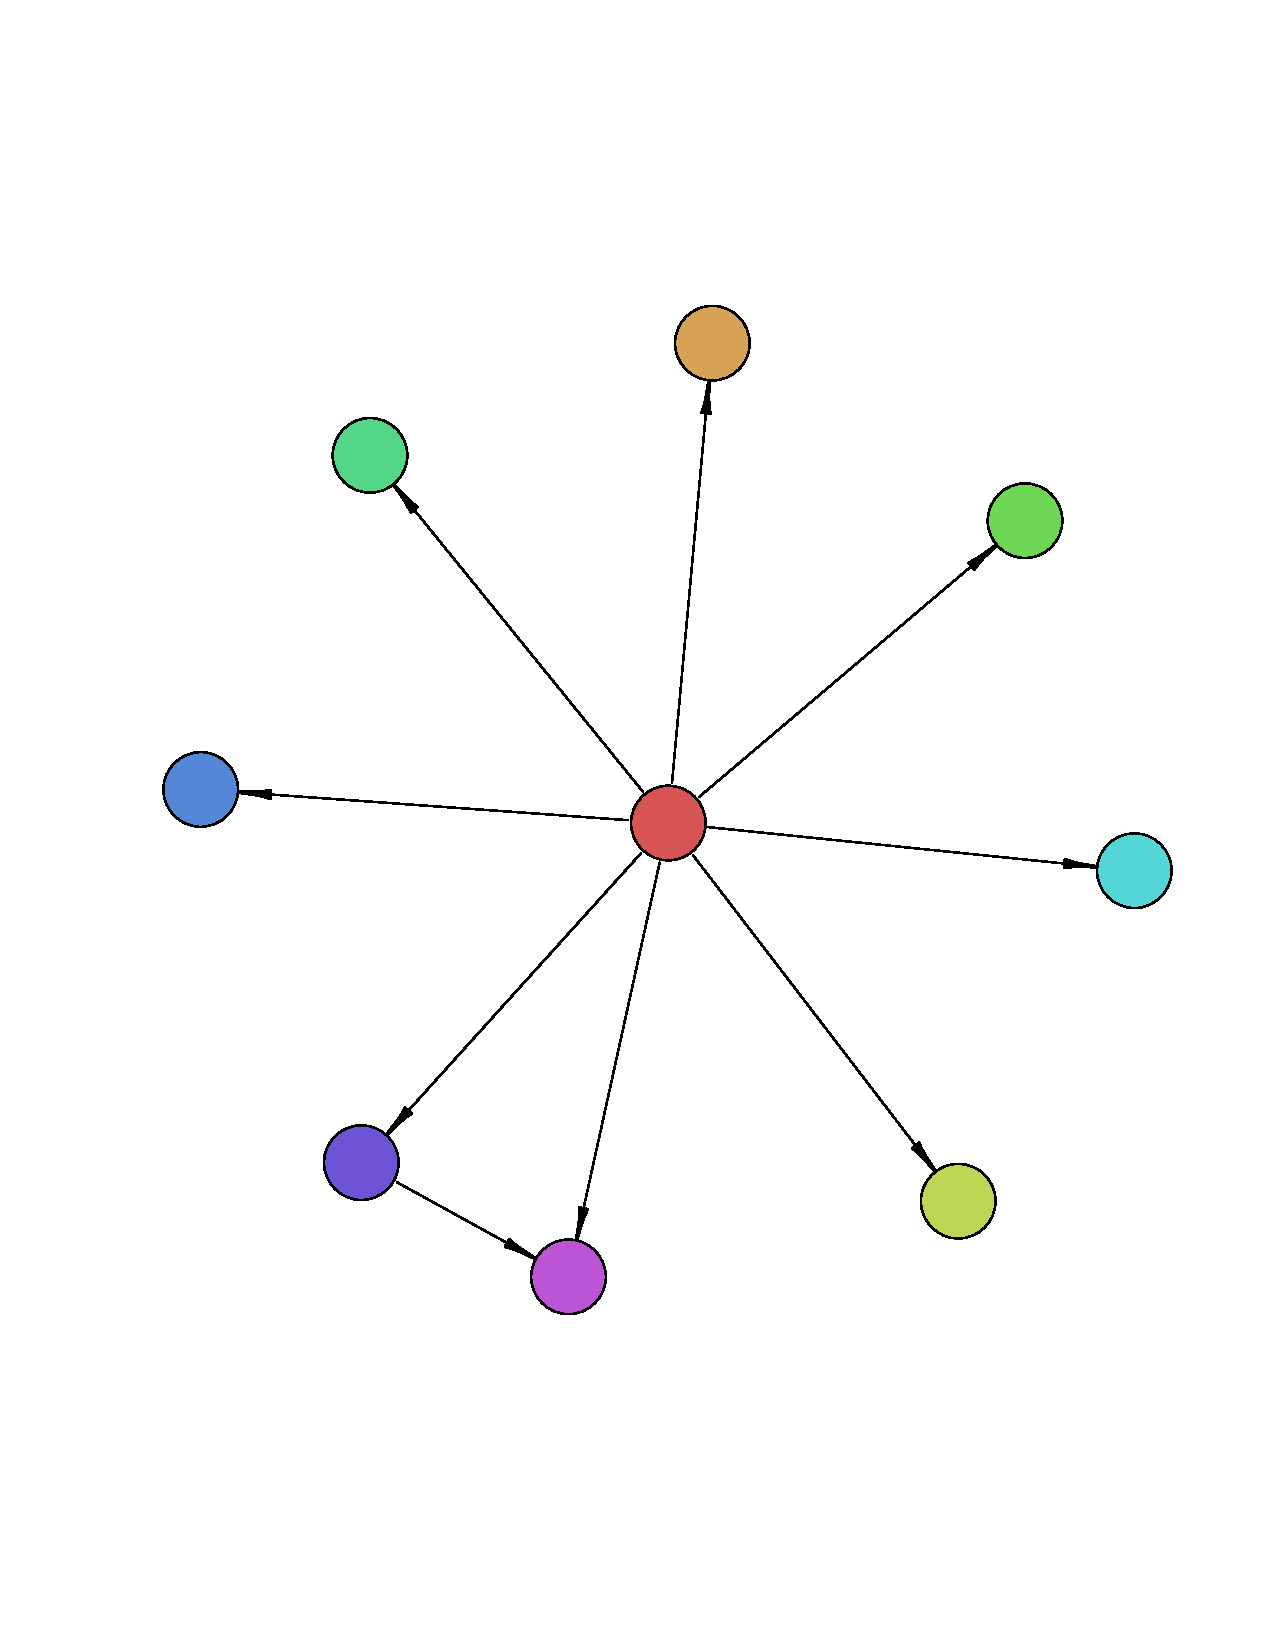
\includegraphics[scale=0.5]{estedef.pdf}
\caption{\small{Ejemplo de una estrella deforme.}} \label{estdef}
\end{figure}


\vspace{0.5cm}

De éste modo, la restricción temporal en las citaciones nos está diciendo que cualquier nodo que aparece en $t_{n}$ puede formar un vínculo con cualquier nodo que hubiese aparecido en $t_1, t_2, t_3, ...t_{n-1}$, de modo que no siempre la estructura de estrella simple (sin ciclos) se mantiene.


\vspace{0.5cm}

De acuerdo con la teoría, las evolución de las redes de citación se da por dos vías: \emph{i.)} vinculación preferencial \citep{Barabasi1, SollaPrice} y \emph{ii.)} ``quién pega primero'' o ``la importancia de ser primicia'' \citep{Newman5, Salazar1}. En la primera vía los artículos con más citas en $t_0$ tienen más probabilidad de recibir una cita en $t_1$ que aquellos que no tienen citas o tienen menos citas. En la segunda vía {\it``los artículos con ventajas tempranas en número de citas las conservarán por la mayor probabilidad de ser citados en nuevos artículos''} \citep[pág. 45]{Salazar1}. Siguiendo una o ambas vías, las citas tienden a agruparse alrededor de un conjunto de artículos que generan la topología tipo estrella deforme dado que las redes de citaciones presentan una estructura jerarquizada \citep{Barabasi2, Ravasz}.


\section{Análisis}
En esta sección vamos a proceder a clasificar la red de acuerdo a estadísticas que traerán luz sobre su topología, principalmente buscaremos determinar si la red estudiada es un mundo pequeño o no. Dado que el objetivo principal de éste estudio es evaluar algoritmos, lo único que buscamos al realizar una descripción topológica de la red es aplicar estadísticas que nos permitan entender la estructura subyacente de la red, así que no se trata entender su proceso de formación estructural (lo cual queda encomendado a próximas publicaciones). Después se estudiarán los resultados entregados por cada algoritmo, y finalmente se realizará la evaluación de los algoritmos.

\subsection{Características Topológicas} \label{TopoRed}
En primer lugar, vamos a examinar algunas estadísticas de la red, usando la base de datos de manera anual acumulada\footnote{Es decir, en el año inicial se contarán las citas de 1976 (por ser el año inicial), para 1977 contaremos las citas de 1977 más las de 1976, para 1978, entonces, se contarán las de 1978 más 1977 más 1976, y así de forma subsiguiente para cada año.} y la base total.

\vspace{0.5cm}

El cuadro \ref{c4} muestra la evolución de estadísticas claves para entender la topología de la red, el diámetro, la densidad, el camino de longitud promedio (A.P.L.\footnote{Siglas del inglés ``average path length''.}) y el coeficiente de agrupación (C.C.\footnote{Siglas del inglés ``clustering coefficient''.}) de la red usando los datos en forma acumulada.


%\vspace{0.5cm}
\begin{table}[h!]
\centering
\resizebox{16cm}{!} {
\begin{tabular}{ccccccccccc}
\textbf{Año} & \textbf{Diámetro} & \textbf{Densidad} &\textbf{A.P.L.} & \textbf{C.C.} & \textbf{Año} & \textbf{Diámetro} & \textbf{Densidad} & \textbf{A.P.L.} & \textbf{C.C.} \\ \hline 
1976 & 1& $0.053$&$1$ & $0.125$&1995 &9 &$6.5 \times 10^{-3}$ & $3.05$&$0.02$\\
1977 & 2& $0.028$&$1.11$ &$0.043$ &1996&9 &$5.4 \times 10^{-3}$ & $3.16$&$0.018$\\
1978 & 2& $0.020$&$1.16$ &$0.045$ &1997 & 9& $4.5 \times 10^{-3}$& $3.31$&$0.016$\\
1979 & 2& $0.014$&$1.21$ &$0.067$ &1998 &10 &$3.8 \times 10^{-3}$ & $3.48$&$0.015$\\
1980 & 4& $0.0096$&$1.35$ &$0.061$ &1999 & 10&$3.2 \times 10^{-3}$ & $3.61$&$0.014$\\
1981 & 4& $0.0084$&$2.42$ &$0.061$ &2000 &11 & $2.7 \times 10^{-3}$& $3.73$&$0.014$\\
1982 & 5& $0.0063$&$2.51$ &$0.055$ &2001 & 11&$2.4 \times 10^{-3}$ & $3.87$&$0.013$\\
1983 & 5& $0.0054$&$1.67$ &$0.054$ &2002 &12 &$2 \times 10^{-3}$ & $4$&$0.013$\\
1984 & 5& $0.0041$&$1.72$ &$0.044$ &2003 &12 & $1.8 \times 10^{-3}$& $4.09$&$0.012$\\
1985 & 6& $0.0033$&$1.83$ &$0.040$ &2004 & 12&$1.5 \times 10^{-3}$ & $4.18$&$0.011$\\
1986 & 6& $0.0028$&$1.98$ &$0.040$ & 2005&12 &$1.3 \times 10^{-3}$ & $4.25$&$0.01$\\
1987 & 8& $0.0024$&$2.13$ &$0.038$ &2006& 12&$1.1 \times 10^{-3}$ & $4.29$&$0.09$\\
1988 & 8& $0.0020$&$2.32$ & $0.037$&2007 &14 &$1 \times 10^{-3}$ & $4.34$&$0.009$\\
1989 & 8& $0.0017$&$2.41$ &$0.035$ &2008 &18 &$9.2 \times 10^{-5}$ & $4.49$&$0.009$\\
1990 & 8& $0.0015$&$2.49$ &$0.034$ &2009 & 16&$8.3 \times 10^{-5}$ & $4.56$&$0.008$\\
1991 & 8& $0.0012$&$2.67$ &$0.031$ &2010 &16 & $7.6 \times 10^{-5}$& $4.64$&$0.08$\\
1992 & 8& $0.0010$&$2.76$ &$0.028$ &2011 &16 & $6.8 \times 10^{-5}$& $4.69$&$0.008$\\
1993 & 8& $0.009$&$2.87$ &$0.026$ & 2012 &16 & $6.2 \times 10^{-5}$& $4.73$ & $0.008$\\
1994 & 8& $7.9 \times 10^{-3}$&$2.96$ &$0.023$ &2013 &16 & $5.7 \times 10^{-5}$& $4.78$& $0.007$\\ \hline
\end{tabular}
}
\caption{\small{Estadísticas básicas de la red usando los datos de forma acumulada. Construcción propia}.}
\label{c4}
\end{table}

\vspace{0.5cm}

El diámetro de un grafo está definido como la mayor distancia entre un par de nodos $n$ en la red. El diámetro representa el tamaño del grafo y permite saber qué tan grande es. De acuerdo con \cite{Watts} una red ``mundo pequeño'' tiene un diámetro no mayor a 6. La densidad mide qué tan disperso --o denso-- es un grafo. Decimos que un grafo es denso si el número de aristas presentes es cercano al número máximo de aristas potenciales, y es disperso sí el número de aristas presentes está alejado del número máximo de aristas potenciales. Para un grafo denso, la medida toma un valor de 1 (o cercano a uno) mientras que para grafos dispersos estará más cercana a cero. Por otro lado, la longitud promedio de los caminos es la media de las distancias entre todos los pares de nodos, es decir, la separación típica entre pares de nodos. Esta medida --junto con el diámetro-- sirve para contrastar la hipótesis de \cite{Watts}, si a medida que la red recibe más nodos su A.P.L. se hace más pequeña, entonces, se trata de un mundo pequeño. Finalmente, el coeficiente de agrupación es la proporción media de pares de vecinos de un nodo que también son vecinos entre sí, es decir, es el número de enlaces que de verdad existen entre los vecinos de un nodo $i$, y la máxima cantidad posible. Al igual que con la densidad, toma el valor de 1 sí la cantidad de enlaces entre vecinos es igual a la máxima posible y toma el valor de 0 si no coinciden.


\vspace{0.5cm}

Sin duda el diámetro y la mayor distancia entre cualquier par de nodos de la red (A.P.L.) revelan que la red estudiada no es un ``mundo pequeño''. Podemos entender la red entonces, como muy separada en términos de nodos y vínculos formados, es decir, existen pocos vínculos para el número de nodos existentes, de hecho, sólo se formaron el $0.0056\%$ de todos los vínculos posibles\footnote{Para encontrar el número máximo de vínculos posibles multiplicamos el número de nodos total por le número de nodos total menos uno: $n(n-1)$ \citep{Newman6}.}. La densidad confirma que a medida que aparecen nuevos nodos, la red se hace más dispersa, lo que contrasta con el coeficiente de clustering (C.C.), donde la probabilidad de que se formen cierres triádicos a medida que son añadidos nuevos nodos y son formados nuevos vínculos a la red tiende a cero.

\vspace{0.5cm}

La figura \ref{f7} nos muestra que los vértices de mayor grado están conectados con vértices cuyo grado también es alto, mientras que los vértices de grado relativamente bajo tienden a conectarse con ambos tipos de vértices (de grado alto y bajo), es decir, los nodos de grado alto se vinculan a otros nodos de grado alto. En términos de citas, entendemos que los artículos muy citados que no pertenecen al núcleo están vinculados a artículos también muy citados\footnote{Con el núcleo nos referimos a los artículos que pertenecen al libro de \citep{Lucas2}}.

\begin{figure}[h!]
\centering
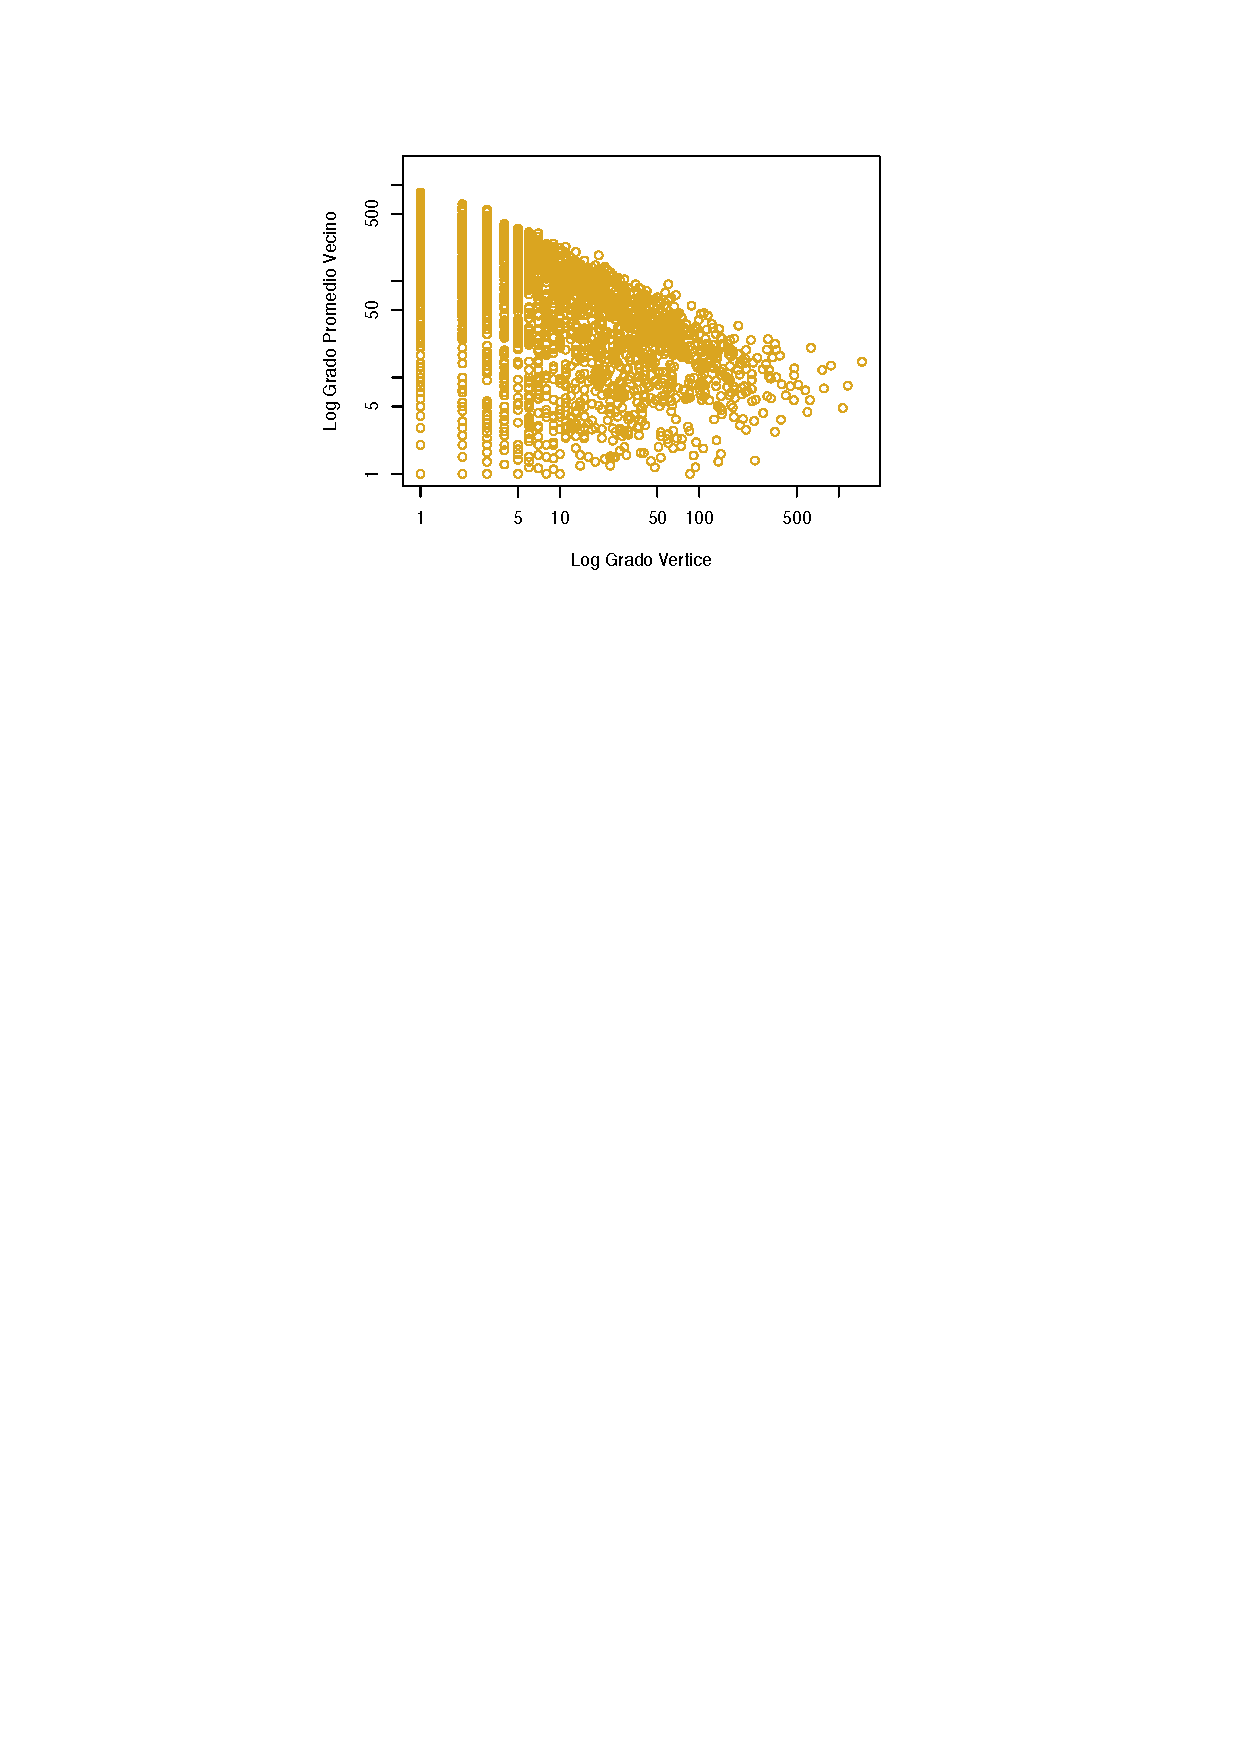
\includegraphics{Log.pdf}
\caption{\small{Grado promedio de vecinos vs grado del vértice. Construcción propia.}} 
\label{f7}
\end{figure}

La figura \ref{f8} muestra la distribución de probabilidad de la red. Se confirma entonces lo planteado por \cite{SollaPrice} y \cite{Albert}: las redes de citas se comportan de acuerdo a una distribución de ley de potencia. Además, confirma lo que hemos observado en las estadísticas anteriores: no todos los nodos tienen el mismo grado y además, muy pocos nodos tienen un grado muy alto, es decir, es mucho más probable recibir pocas citas (o no tenerlas) que tener muchas citas.



\begin{figure}[h!]
\centering
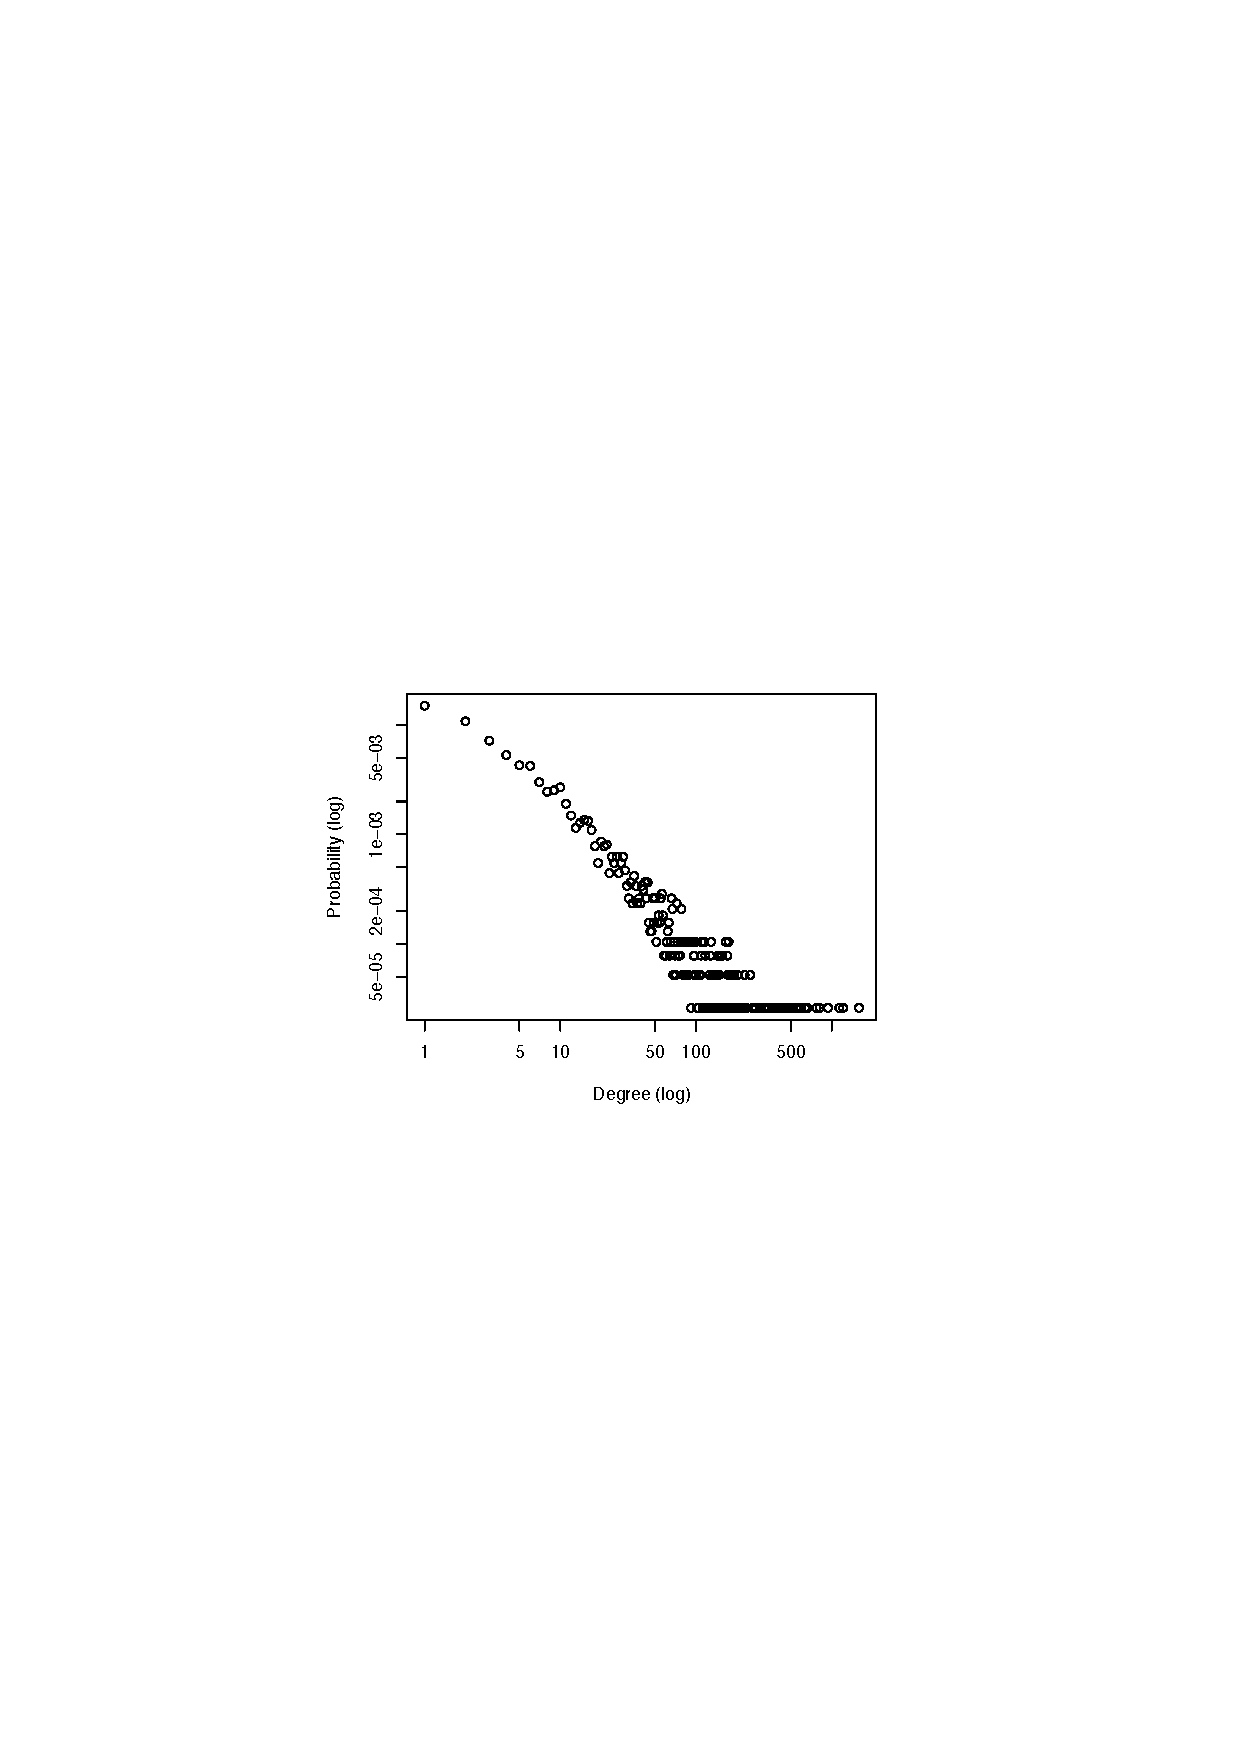
\includegraphics{Dist.pdf}
\caption{\small{Distribución de probabilidad. Construcción propia.}} 
\label{f8}
\end{figure}


\vspace{0.5cm}
Una idea interesante que surge a partir de las figuras \ref{f7} y \ref{f8} concierne a la estructura topológica: la red podría resumirse como cúmulos de estrellas conectadas una a otras por medio de puentes.

\subsection{Características y Evaluación de los Módulos}
Lo primero que vamos a apreciar de cada algoritmo es el número de particiones que realiza sobre la red total (ver cuadro \ref{c3} para conocer el número de nodos y vínculos sobre los que cada algoritmo ``corrió''). A continuación se muestra el número de comunidades encontradas por cada algoritmo\footnote{Además de las 483 comunidades encontradas por el algoritmo de \cite{Girvan1, Girvan2}, el algoritmo encontró 20.131 nodos de intermediación en la red que no son contadas como comunidades ni se incluyen dentro de las comundiades econtradas.}.

\begin{table}[h!]
\centering
%\resizebox{12cm}{!} {
\begin{tabular}{cccccc}
\textbf{Algoritmo} & \textbf{Comunidades} \\ \hline 
   \cite{Blondel} & 102  \\
   \cite{Clauset} &  236 \\
   \cite{Girvan1, Girvan2}  & 483\\
    \cite{Pons}  & 1165 & \\
    \cite{Raghavan}  & 940\\
    \cite{Rosvall1} & 1616 \\ \hline
\end{tabular}
%}
\caption{\small{Número módulos encontrados por algoritmo en la red total}.}
\label{c5}
\end{table}

En general, todos los algoritmos --aunque difieren de las comunidades encontradas-- concuerdan en un hecho: existen estrellas (incluidas díadas y tríadas) que no se conectan con ningún componente de la red salvo con sus pares adyacentes.  En total son 47 comunidades que se encuentran aisladas del resto de la red, cumpliendo siempre una regularidad: la diferencia entre el número de nodos y de vínculos de cada uno de estos componentes es igual a 1, de modo que éste tipo de módulo puede ser definido como $G=(V,E)$ donde $E=V-1$.

\vspace{0.5cm}

El cuadro \ref{c7} muestra el total de componentes aislados y el número de veces que éstos aparecen en la red. Es evidente que se trata de un conjunto de nodos cuyo grado máximo es 87 y el mínimo es 1.

\vspace{0.5cm}

\begin{table}[h!]
\centering
%\resizebox{12cm}{!} {
\begin{tabular}{cccc}
\textbf{Componente} & \textbf{Frecuencia} &\textbf{Nodos} & \textbf{Vínculos} \\ \hline 
1 & 1 & 87 & 86  \\
2 & 1 & 11 &  10 \\
3 & 1 & 9  & 8\\
4 & 1 &  6  & 5  \\
5 & 4 &  4  & 3\\
6 &  8 &  3 & 2 \\ 
7 & 31  &  2 & 1 \\\hline
\end{tabular}
%}
\caption{\small{Resumen composición de estrellas aisladas}.}
\label{c7}
\end{table}

\vspace{0.5cm}
El cuadro \ref{c8} muestra los cinco módulos más grandes (en términos de nodos) y la cantidad de vínculos por comunidad. Es posible notar la similitud en los cortes --respecto al tamaño de las comunidades-- entre algunos algoritmos. Por ejemplo, en el componente 1, los algoritmos de \cite{Clauset} y \cite{Pons} tienen aproximadamente el mismo número de nodos. En el componente 2 los algoritmos de \cite{Blondel} y \cite{Pons} sin similares en el número de nodos y de vínculos intra-comunidad. En los módulos 3, 4 y 5, son similares los cortes de \cite{Blondel} y \cite{Clauset} y de \cite{Raghavan} y \cite{Rosvall1}. La similaridad entre algunos de los cortes de algunos algoritmos de debe a los métodos usados para encontrar los módulos, por ejemplo, \cite{Blondel} y \cite{Clauset} en sus cortes buscan maximizar la modularidad, \cite{Pons}, \cite{Raghavan} y \cite{Rosvall1} buscan las comunidades utilizando un caminante aleatorio y \cite{Girvan1, Girvan2} eligen la mejor partición de acuerdo a la mayor intermediación\footnote{Sobre el funcionamiento de cada algoritmo consultar la sección \ref{EvAl}.}.

\vspace{0.5cm}
\begin{table}[h!]
\centering
\resizebox{16cm}{!} {
\begin{tabular}{lcccccc}
\textbf{Algoritmo / Componente} & 1 & 2 & 3 & 4 & 5\\ \hline 
   \cite{Blondel} &$4552 (7209)$& $3814 (8480)$ & $3469 (7486)$ & $3119 (5544)$ & $2673 (3794)$ \\
   \cite{Clauset} &$6055 (16227)$&$5356 (9404)$&$4716 (8083)$&$3789 (6716)$&$3462 (5243)$\\
   \cite{Girvan1, Girvan2}  &$15969 (26281)$&$987(1056)$&$978 (1604)$&$452(754)$&$580 (736)$\\
    \cite{Pons}    &$6020 (12436)$&$3690 (8574)$ &$1729 (3060)$&$1142 (1438)$&$1129 (1283)$\\
    \cite{Raghavan}  &$11581 (27577)$&$961 (1168)$&$628 (647)$&$615 (616)$&$558 (1911)$\\
    \cite{Rosvall1} &$786 (2238)$&$575 (575)$&$546 (817)$&$502 (1802)$&$443 (442)$\\ \hline
\end{tabular}
}
\caption{\small{Tamaño en nodos de los cinco componentes más grandes. (Número de vínculos intra-comunidad)}.}
\label{c8}
\end{table}

\vspace{0.8cm}

El cuadro \ref{c9} muestra el grado máximo que tiene un nodo en cada componente por algoritmo. Los valores con colores idénticos (excepto el negro) representan a los mismos nodos, es decir, en todos los cortes realizados por los algoritmos, con base en las cinco comunidades más grandes, hay en común 6 nodos --o artículos-- en los cortes realizados por cada algoritmo. Esto da evidencia de la estructura jerarquizada de la red, pues las cinco comunidades más grandes se ordenan al rededor de 6 artículos muy citados que son comunes en todos los cortes. 

\vspace{0.5cm}

Esto muestra que la comunidad de los nuevos economistas clásicos no ha logrado ponerse de acuerdo respecto a qué vertiente seguir para desarrollar su paradigma, dado que, de existir un acuerdo, el número de comunidades sería menor (en todos los algoritmos), pues los nodos estarían más conectados y las comunidades que surgirían --como alternativa al componente más conexo-- no tendrían nodos con grados tan altos. 

\vspace{0.5cm}
\begin{table}[h!]
\centering
\begin{tabular}{lcccccc}
\textbf{Algoritmo / Grado} & 1 & 2 & 3 & 4 & 5\\ \hline 
   \cite{Blondel} &{\color{Magenta2}438}& {\color{RoyalBlue1} 939} & {\color{Red2} 342}&{\color{Tan1}859}&{\color{Purple3} 627} \\
  
   \cite{Clauset} &{\color{RoyalBlue2}1130}&{\color{Magenta2}498}&{\color{Purple3} 807}&969&435\\
  
   \cite{Girvan1, Girvan2} &{\color{RoyalBlue2} 1050}&{\color{Tan1}876}&{\color{SpringGreen4} 766}&323&{\color{Purple3} 478}\\
  
    \cite{Pons}    &{\color{Red2} 390}&{\color{RoyalBlue1} 851} &{\color{Magenta2}323} &{\color{Purple3}536}&{\color{SpringGreen4}604}\\
  
    \cite{Raghavan}  &{\color{RoyalBlue1}1258}&{\color{SpringGreen4} 606}&{\color{Tan1}597}&{\color{Magenta2}235}&88\\
  
    \cite{Rosvall1} &{\color{Red2} 251}&{\color{SpringGreen4} 573}&$419$&$158$&{\color{Purple3} 440}\\ \hline

\end{tabular}
\caption{\small{Nodo de máximo grado por comunidad}.}
\label{c9}
\end{table}

\vspace{0.5cm}

De forma puntual, en la tabla \ref{c9}, los artículos en común entre los cinco componentes más grandes por algoritmo son: \cite{Kydland} (Azul), \cite{Lucas1} (verde), \cite{Hall} (magenta), \cite{Blanchard} (púrpura), \cite{Rudebusch} (rojo) y \cite{Granger} (amarillo).


\vspace{0.5cm}
Finalmente, evaluamos los algoritmos con las medidas propuestas en la sección \ref{Criterio}. El cuadro \ref{c6} muestra el resultado de cada medida para cada algoritmo. Es posible observar que las mejores medidas las tienen el algoritmo de \cite{Blondel} y el de \cite{Clauset} cuyos cortes --de las cinco comunidades más grandes-- tienen 4 nodos en común. Algo curioso respecto a estos dos algoritmos es que ambos buscan maximizar la modularidad al momento de realizar los cortes, esto explica porqué tienen las mejores medidas de modularidad. Por otro lado, con la métrica \emph{conductancia}, entendemos que ambos algoritmos encuentran las comunidades más densas internamente y alejadas con el resto de la red dentro del conjunto de algoritmos evaluados.

\vspace{0.5cm}
\begin{table}[h!]
\centering
%\resizebox{9cm}{!} {
\begin{tabular}{cccccc}
\textbf{Algoritmo} & \textbf{Modularidad}  & \textbf{Conductancia} \\ \hline 
   \cite{Blondel} & $0.7114$  & $0.1433$\\
   \cite{Clauset} &  $0.7005$ & $0.1434$\\
   \cite{Girvan1, Girvan2}  & $0.1594$ & $0.2661$\\
    \cite{Pons}  & $0.6430$  & $0.2594$ \\
    \cite{Raghavan}  & $0.5816$  & $0.2216$\\
    \cite{Rosvall1} & $0.6066$ & $0.3847$\\ \hline
\end{tabular}
%}
\caption{\small{Modularidad y conductancia por algoritmo}.}
\label{c6}
\end{table}

%\subsection{Resultados}

\section{Conclusiones}
Luego de realizar una serie de acercamientos a la red estudiada hemos podido entender parte de la topología de la red y su estructura subyacente. En primer lugar, es evidente que no se trata de un mundo pequeño. Esto nos habla de lo separada --en términos de nodos-- que se encuentra la Nueva Economía Clásica (de ahora en adelante NEC) pese a tener una metodología definida y bastante tiempo construyendo sus programas de investigación \citep{Salazar1}. 

\vspace{0.5cm}
Esta separación en la red puede deberse a la clasificación del libro de \cite{Lucas2} de donde obtuvimos la base para construir las citas, dado que está dividido en seis secciones que tratan distintos frentes de investigación que evidentemente no convergen al uso de las mismas citas\footnote{Es evidente debido a que si convergiesen al uso de las mismas citas sin duda se trataría de un mundo pequeño.}. En términos ontológicos podemos entender dicha separación en la forma en que la NEC se desarrolla: aunque la metodología los une, las técnicas los separan. Es decir, un científico ocupa un lugar en la NEC más por su tecnología que por su metodología. Esto puede verse reflejado en la existencia de mínimo 102 y máximo 1616 comunidades (ver cuadro \ref{c5}) y por la conformación de los nodos de mayor grado en las 5 comunidades más grandes (ver cuadro \ref{c9}). Si las técnicas unieran a la NEC los nodos de grado más alto conformarían un único componente --asumiendo los nodos de mayor grado como los artículos que más aceptación tuvieron en el panorama científico y por lo tanto sus aportes subyacentes son los más usados en el paradigma--, sin embargo, la mayoría de artículos con grados altos no están conectados de forma fuerte con sus pares de grado alto.


\vspace{0.5cm}

El estudio de las comunidades resultó muy diciente en la organización de las redes de citas en la economía. Aunque los algoritmos diferían en el número de módulos y el tamaño de los módulos (en términos de nodos), en general los cinco clusters más grandes para cada corte de cada algoritmo resultaron conteniendo al menos el mismo conjunto de artículos muy citados --o nodos con grados altos-- (ver cuadro \ref{c9}).

\vspace{0.5cm}

Respecto a la evaluación de los algoritmos, por un lado, las métricas usadas dan muestra la efectividad de los algoritmos de \cite{Blondel} y \cite{Clauset} ambos del tipo ``densidad''. Por lo tanto nuestra hipótesis es rechazada. Por otro lado, la razón por la que el algoritmo de \cite{Girvan1, Girvan2} resultó tan mal ``parado'' se debe a la clasificación de los nodos de intermediación que hace el algoritmo, es decir, al correr el algoritmo de \cite{Girvan1, Girvan2} detecta los nodos con mayor intermediación y los substrae de las comunidades, evitando que estos sean ``contados'' dentro de algún módulo, así, por ejemplo, al evaluar la modularidad sobre sus cortes, la organización de la red aleatoria diferirá mucho de la red original.

\vspace{0.5cm}

Por lo tanto, para la detección de comunidades en redes de citación se recomienda el uso del algoritmo de \cite{Blondel} o \cite{Clauset}, en el caso que se desee encontrar los particionamientos en la red; por otro lado, para la detección de los nodos intermediarios se recomienda el uso del algoritmo de \cite{Girvan1, Girvan2}

\vspace{0.5cm}

No obstante, considero que para estudios ontológicos de la economía con redes de citas utilizar varios algoritmos y compararlos resulta siendo muy enriquecedor para entender aún mejor la organización de la ciencia que usando solo uno, pues permite contrastar por varios caminos la conformación de los módulos y entender de una forma más amplia el panorama científico. En el caso del algoritmo de \cite{Girvan1, Girvan2}, su utilidad se ve reflejada en análisis de intermediación y no de conglomerados.


\vspace{0.5cm}

Como remanente de éste artículo se propone el mismo análisis para la Nueva Economía Keynesiana (NEK de ahora en adelante) y para la red conjunta (NEC y NEK). De esta manera el estudio de la historia empírica tomará más valor y sustento para falsear las historia que nos fue contada respecto a la caída de la NEK y ascensión de la NEC. Queda además encomendada la labor de seguir construyendo las redes de citas para los siguientes diez años e intentar predecir --desde el análisis de redes complejas-- el rumbo que tomarán la ciencia económica.

\newpage
\bibliographystyle{apalike}
\bibliography{Tesis.bib}
%\begin{thebibliography}{}
%\bibitem{Blondel} Blondel, V., Guillaume, J-P., Lambiotte, R. \& Lefebvre, E. (2008). {\it ``Fast unfolding of communities in large networks''.} Journal of Statistical Mechanics: Theory and Experiment (10), P10008 (12pp).
%\bibitem{Clauset} Clauset, A., Newman, M. \& Moore, C. (2004). {\it ``Finding community structure in very large networks}. Physical Review. E 70, 066111.
%\bibitem{Girvan1} Girvan, M \& Newman, M. (2002). {\it ``Community structure in social and biological networks''}. Proceedings of the National Academy of Science, 99(12), 7821-7826.
%\bibitem{Girvan2} Girvan, M \& Newman, M. (2002). {\it ``Finding and evaluating community structure in networks''}. Physical Review. E. Statistical, Nonlinear and Soft Matter Physics, 69(2), 026113.
%\bibitem{Kuhn} Kuhn, T. S. (1962). {\it ``The structure of scientific revolutions''}. Chicago University Press.
%\bibitem{Labatut} Labatut, V. \& Balasque, J-M. (2011). {\it ``Detection and interpretation of community in complex networks, methods and practical application''}.  Computational social networks analysis: trends, tools and research advantages, Springer, Computer and Communication Netwroks.
%\bibitem{Leskovec} Leskovec, J. (2007). {\it ``Dynamics on large networks''} (Tesis de Doctorado). Carnegie Mellon University.
%\bibitem{Leskovecetal1} Leskovec, J., Lang, K. J.
%\bibitem{Leskovecetal2} 
%\bibitem{Pons} Pons, P. \& Latapy, M. (2005). {\it ``Computing communities in large networks using random walks (long version)''}. ePrint arXiv:physics/0512106.

%\bibitem{Raghavan} Raghavan, U. N., Albert, R. \& Kumara, S. (2007). {\it ``Near linear time algorithm to detect community structures in large-scale networks''}. Physical Review. E. Statistical, Nonlinear and Soft Matter Physics, 76:036106.
%\bibitem{Rosvall1} Rosvall, M., Axelsson, D. \& Bergstrom, C. (2008). {\it ``Maps of random walks on complex networks reveal community structure''}. PNAS 105, 1118.
%\bibitem{Rosvall2} Rosvall, M., Axelsson, D. \& Bergstrom, C. (2009). {\it `` The map equation''}. Eur. Phys. J. Special Topics 178, 13.
%\bibitem{Rosvall3} Rosvall, M. \& Bergstrom, C. (2009). {\it ``Mapping change in large network''}. PLoS ONE 5(1): e8694.
%\bibitem{Salazar1} Salazar, B. \& Otero. D. (2015). {\it ``La revolución de los nuevos clásicos: redes, influencia y metodología''}. Revista de Economía Institucional 17, 32, pp. 36-69.
%\bibitem{Salazar2} Salazar, B., Otero. D. \& Escandón J. C. (2016). {\it ``Consenso y divergencia en la revolución de los nuevos clásicos'}. Manuscrito.
%\bibitem{Yang}

%\end{thebibliography}
\newpage
\section{Anexos}
En esta sección se presentarán los códigos de las funciones creadas en R para el análisis de las comunidades. Sin embargo, en la página personal de GitHub del autor (https://github.com/Rodato) el lector más interesado encontrará periódicamente nuevas funciones --que no se incluyen en las librerías-- para análisis de redes complejas en R y Python.
\subsection{Función 1}
Función para detectar el número de comunidades, el tamaño de las comunidades y los vínculos intra e inter comunidad por algoritmo.

\vspace{0.5cm}
\lstset{language=R, basicstyle=\footnotesize}
\begin{lstlisting}[frame=single]
inter.intra.edges<-function(G,algorithm) {
  ##definimos el algoritmo a usar:
  #**Tener en cuenta 
  #1=cluster_louvain(); 2=cluster_edge_betweenness(); 
  #3=cluster_walktrap()
  #4=cluster_label_prop(); 5=cluster_fast_greedy(); 6=cluster_infomap()
  
  if(algorithm==1){
    Modu<-cluster_louvain(G)}
  if(algorithm==2){
    Modu<-cluster_edge_betweenness(G)}
  if(algorithm==3){
    Modu<-cluster_walktrap(G)}
  if(algorithm==4){
    Modu<-cluster_label_prop(G)}
  if(algorithm==5){
    Modu<-cluster_fast_greedy(G)}
  if(algorithm==6){
    Modu<-cluster_infomap(G)}
  if(algorithm > 6){
    print("Número no valido de algoritmo")}
  
  
  ##Calculamos el número de comunidades y su tamaño
  Com<-as.data.frame(sizes(Modu))
  ##Extraemos el número de comunidades por membresía
  NoCom<-as.vector(Com$Community.sizes)
  #Comenzamos a extraer los subgrafos
  intra<-vector()
  inter<-vector()
  for(i in 1:length(NoCom)){
    M<-which(membership(Modu)==i)
    sg<-induced.subgraph(G,M)
    c.ec<-ecount(sg) #cantidad de vinculos intra-comunidad
    i.ds<-sum(degree(sg))
    c.vds<-sum(degree(G,M))
    e.esum <-c.vds-i.ds
    
    inter[i]<-e.esum
    intra[i]<-c.ec
  }

  cc<-data.frame(Com,intra,inter)
  print(cc)
}
\end{lstlisting}

\newpage
\subsection{Función 2}
Función para calcular la conductancia.

\vspace{0.5cm}
\lstset{language=R, basicstyle=\footnotesize}
\begin{lstlisting}[frame=single]
Conductance<-function(graph, community.vertices) {
  ## Grafo compuesto únicamente por los vértices que 
  ## pertenecen a la comunidad
  cluster.subgraph <- induced.subgraph(graph, community.vertices)
  
  ## Grado para cada subgrafo
  intra.degree <- graph.strength(cluster.subgraph, mode="all")
  
  ## grado de los nodos de cada comunidad
  community.vertices.degree <- graph.strength(graph, community.vertices,
                                              mode="all")
  
  ## sumamos los grados de todos los nodos 
  community.vertices.degree.total  <- sum(community.vertices.degree)
  intra.degree.total               <- sum(intra.degree)
  
  ## sumos todos lo cruces de vínculos
  inter.edge.sum <- community.vertices.degree.total - intra.degree.total
  
  return(inter.edge.sum / community.vertices.degree.total)
}
\end{lstlisting}


\end{document}
